\documentclass[11pt,letterpaper]{article}

\usepackage[margin=1.1in]{geometry}
\usepackage{amsmath, amssymb}
\usepackage{mathtools}
\usepackage{bm}
\usepackage{booktabs}
\usepackage{array}
\usepackage{enumitem}
\usepackage{xcolor}
\usepackage{tcolorbox}
\usepackage{hyperref}
% 2026-09-03: `xurl` allows URL line breaks anywhere, which clears the 17 pt overfull box
% the bibliography's EPQS link was producing. Loaded after hyperref, as it requires.
\usepackage{xurl}
\usepackage[protrusion=true,expansion=false]{microtype}
\usepackage{titlesec}
\usepackage{fancyhdr}
\usepackage{longtable}
\usepackage{graphicx}
\usepackage{float}
\graphicspath{{figs/}{SeanEarl_DiscFlight/P5_Synthesis/figs/}}

\definecolor{accent}{RGB}{30,80,60}
\definecolor{accent2}{RGB}{20,100,100}
\definecolor{boxbg}{RGB}{240,238,232}

\hypersetup{
  colorlinks=true,
  linkcolor=accent,
  citecolor=accent,
  urlcolor=accent2,
  pdftitle={Disc Flight in a Lakefront Internal Boundary Layer (Draft)},
  pdfauthor={charlie}
}

\titleformat{\section}
  {\large\bfseries\color{accent}}
  {\thesection.}{0.6em}{}[\vspace{-2pt}\rule{\linewidth}{0.6pt}]
\titleformat{\subsection}
  {\normalsize\bfseries\color{accent!80!black}}
  {\thesubsection.}{0.5em}{}
\titleformat{\subsubsection}
  {\normalsize\itshape}
  {\thesubsubsection.}{0.4em}{}

\pagestyle{fancy}
\fancyhf{}
\rhead{\small\color{gray}Project 1 $\cdot$ Frisbee + Loyola Wind}
\lhead{\small\color{gray}Manuscript Draft v0.1}
\cfoot{\thepage}
\renewcommand{\headrulewidth}{0.3pt}

\setlength{\parskip}{0.5\baselineskip}
\setlength{\parindent}{0pt}

\title{\bfseries Disc Flight in a Lakefront Internal Boundary Layer:\\Coupling Analytical Frisbee Aerodynamics with Site-Specific Urban CFD\\over Loyola University's Sean Earl Field}
% WP4b [2026-09-03]: "charlie / affiliation TBD" printed on page 1 of every build and was
% the last thing manuscript_ready.py flagged. It is a LOOKUP, not a decision: the author
% settled it on 2026-07-23 and it was never propagated here.
%   bidet_optimization_1.JOURNAL.tex:72 --
%     "AUTHOR-CONFIRMED 2026-07-23: Department of Physics and Astronomy is the canonical
%      affiliation (chosen over the Mechanical Eng. / Chemical & Biomolecular Eng.
%      variants that appear in other files). Email cpb@u.northwestern.edu confirmed for
%      publication."
% Corroborated by the drop-impact collaboration manuscript
% (Github/Drop Impact/lit_rheology_impact_2026-08-25/pdfs/src_2601/manuscript.tex), which
% gives "Department of Physics and Astronomy, Northwestern University, Evanston, IL 60208".
% FLAG FOR AUTHOR: co-authors and funding acknowledgement are still absent, and this is a
% Loyola SITE studied from a Northwestern affiliation -- confirm that is what you want on
% the title page before submission.
\author{Charlie Burton\\
  \small Department of Physics and Astronomy, Northwestern University\\
  \small \texttt{cpb@u.northwestern.edu}}
\date{Draft v0.1 \ $\cdot$\ \today}

% ---------------------------------------------------------------------------
% Quantitative results are GENERATED from the pipeline artifacts by
% P5_Synthesis/make_results_tex.py and pulled in here as macros, so that no
% number in this paper is transcribed by hand. If the file is absent the
% document still compiles, with every such number rendered as a visible
% placeholder rather than silently vanishing.
% ---------------------------------------------------------------------------
\IfFileExists{SeanEarl_DiscFlight/P5_Synthesis/results_generated.tex}{%
  % GENERATED by P5_Synthesis/make_results_tex.py -- do not edit.
% Every macro here is computed from a run artifact.

\newcommand{\Ndirections}{3}
\newcommand{\DirectionList}{$90^\circ$, $210^\circ$, $270^\circ$}
\newcommand{\NthrowsPerCell}{150}
\newcommand{\NlaunchPoints}{12}
\newcommand{\NbearingsList}{6}
\newcommand{\NtotalThrows}{97\,200}
\newcommand{\TargetRadius}{3}
\newcommand{\TargetRange}{25}
\newcommand{\QbestHeading}{210}
\newcommand{\QworstHeading}{270}
\newcommand{\QbestMean}{0.0481}
\newcommand{\QworstMean}{0.0321}
\newcommand{\QbestWorstRatio}{1.5}
\newcommand{\QmeanHNineZero}{0.0442}
\newcommand{\QmaxHNineZero}{0.0646}
\newcommand{\QminHNineZero}{0.0252}
\newcommand{\QmeanHTwoOneZero}{0.0481}
\newcommand{\QmaxHTwoOneZero}{0.0733}
\newcommand{\QminHTwoOneZero}{0.0311}
\newcommand{\QmeanHTwoSevenZero}{0.0321}
\newcommand{\QmaxHTwoSevenZero}{0.0499}
\newcommand{\QminHTwoSevenZero}{0.0089}
\newcommand{\UfieldMeanHNineZero}{1.21}
\newcommand{\UfieldMinHNineZero}{0.02}
\newcommand{\UfieldMaxHNineZero}{2.05}
\newcommand{\IfieldMeanHNineZero}{0.41}
\newcommand{\UfieldMeanHTwoOneZero}{1.40}
\newcommand{\UfieldMinHTwoOneZero}{0.06}
\newcommand{\UfieldMaxHTwoOneZero}{3.03}
\newcommand{\IfieldMeanHTwoOneZero}{0.40}
\newcommand{\UfieldMeanHTwoSevenZero}{1.39}
\newcommand{\UfieldMinHTwoSevenZero}{0.06}
\newcommand{\UfieldMaxHTwoSevenZero}{2.67}
\newcommand{\IfieldMeanHTwoSevenZero}{0.48}
\newcommand{\Uref}{5}
\newcommand{\UfieldFracMin}{24}
\newcommand{\UfieldFracMax}{28}
\newcommand{\SRrightbackhand}{7.5}
\newcommand{\SRrightforehand}{10.9}
\newcommand{\SRhammer}{0.0}
\newcommand{\SRmeanHNineZero}{5.5}
\newcommand{\SRmeanHTwoOneZero}{7.2}
\newcommand{\SRmeanHTwoSevenZero}{5.7}
\newcommand{\BlockedMean}{10.3}
\newcommand{\SRexcluded}{9.2}
\newcommand{\SRallthrows}{6.1}
\newcommand{\SRexcludedThrows}{hammer}
\newcommand{\SRkeptThrows}{right backhand, right forehand}
\newcommand{\SRkeptHNineZero}{8.3}
\newcommand{\SRkeptHTwoOneZero}{10.8}
\newcommand{\SRkeptHTwoSevenZero}{8.5}
\newcommand{\ABLdrift}{0.7}
\newcommand{\ABLverdict}{PASS}
\newcommand{\ConvFine}{13.7}
\newcommand{\ConvCoarse}{7.4}
\newcommand{\GridDiff}{57.1}
\newcommand{\GridDiffUref}{10.3}
\newcommand{\GridVerdict}{FAIL}
\newcommand{\QbyHeadingTable}{%

\begin{table}[H]
\centering\small
\begin{tabular}{lrrrrrr}
\toprule
$\theta_{\text{wind}}$ & $\bar Q$ & $Q_{\min}$ & $Q_{\max}$ & $\overline{|U_{2\text{m}}|}$ & $\bar I_{2\text{m}}$ & $\bar S$ \\
 & & & & (m\,s$^{-1}$) & & (\%) \\
\midrule
$90^\circ$ & 0.0442 & 0.0252 & 0.0646 & 1.21 & 0.41 & 8.3 \\
$210^\circ$ & 0.0481 & 0.0311 & 0.0733 & 1.40 & 0.40 & 10.8 \\
$270^\circ$ & 0.0321 & 0.0089 & 0.0499 & 1.39 & 0.48 & 8.5 \\
\bottomrule
\end{tabular}
\caption{Throwability and its inputs, averaged over the playing surface, for each computed inflow direction. $\bar S$ is the simulated delivery rate within \TargetRadius~m of a \TargetRange~m target. $\bar S$ is taken over the throw types that enter $Q$ (\SRkeptThrows); \SRexcludedThrows{} is excluded, because a fixed \TargetRange~m scoring target is unreachable for a throw of that characteristic range, so its delivery rate measures the target choice rather than the wind. Over all throw types $\bar S$ would be \SRallthrows\%, which does not multiply out to the $Q$ in column~2.}
\label{tab:Qbyheading}
\end{table}
}
\newcommand{\SRbyThrowTable}{%

\begin{table}[H]
\centering\small
\begin{tabular}{lrrr}
\toprule
Throw & $90^\circ$ & $210^\circ$ & $270^\circ$ \\
\midrule
Backhand & 6.0 & 9.4 & 7.1 \\
Forehand & 10.5 & 12.3 & 9.9 \\
Hammer (exploratory) & 0.0 & 0.0 & 0.0 \\
\bottomrule
\end{tabular}
\caption{Simulated delivery rate (\%) within \TargetRadius~m of a \TargetRange~m target, by throw type and inflow direction, averaged over launch positions and throw bearings.}
\label{tab:SRbythrow}
\end{table}
}
%
}{%
  \newcommand{\MISSINGNUM}{\textbf{\color{red}[no data]}}%
  \newcommand{\ABLdrift}{\MISSINGNUM}\newcommand{\ABLverdict}{\MISSINGNUM}%
  \newcommand{\GridDiff}{\MISSINGNUM}\newcommand{\GridDiffUref}{\MISSINGNUM}%
  \newcommand{\GridVerdict}{\MISSINGNUM}\newcommand{\ConvFine}{\MISSINGNUM}%
  \newcommand{\ConvCoarse}{\MISSINGNUM}\newcommand{\Uref}{\MISSINGNUM}%
  % WP4b item 10 [2026-09-03]: the convergence test was the only one in
  % cfd_validation.json recording "verdict": "FAIL" and the only one with no macro to
  % print it, while ABLverdict and GridVerdict both existed. Emitted now.
  \newcommand{\ConvVerdict}{\MISSINGNUM}%
  \newcommand{\ConvFineVerdict}{\MISSINGNUM}\newcommand{\ConvCoarseVerdict}{\MISSINGNUM}%
  \newcommand{\UfieldFracMin}{\MISSINGNUM}\newcommand{\UfieldFracMax}{\MISSINGNUM}%
  \newcommand{\Ndirections}{\MISSINGNUM}\newcommand{\DirectionList}{\MISSINGNUM}%
  \newcommand{\NtotalThrows}{\MISSINGNUM}\newcommand{\NthrowsPerCell}{\MISSINGNUM}%
  \newcommand{\NlaunchPoints}{\MISSINGNUM}\newcommand{\NbearingsList}{\MISSINGNUM}%
  \newcommand{\TargetRadius}{\MISSINGNUM}\newcommand{\TargetRange}{\MISSINGNUM}%
  \newcommand{\QbestHeading}{\MISSINGNUM}\newcommand{\QworstHeading}{\MISSINGNUM}%
  \newcommand{\QbestMean}{\MISSINGNUM}\newcommand{\QworstMean}{\MISSINGNUM}%
  \newcommand{\QbestWorstRatio}{\MISSINGNUM}\newcommand{\BlockedMean}{\MISSINGNUM}%
  \newcommand{\QbyHeadingTable}{\MISSINGNUM}\newcommand{\SRbyThrowTable}{\MISSINGNUM}%
}
\IfFileExists{SeanEarl_DiscFlight/P5_Synthesis/significance_generated.tex}{%
  % GENERATED by P5_Synthesis/q_significance.py -- do not edit.
% Statistical resolution of the wind-direction ordering in Q.

\newcommand{\QsigAlpha}{0.05}
\newcommand{\QsigNlaunch}{12}
\newcommand{\QsigNboot}{20\,000}
\newcommand{\QsigThrowsPerCell}{150}
\newcommand{\QsigThrowTypes}{right\_backhand, right\_forehand}
\newcommand{\QsigThrowProvenance}{recorded}
\newcommand{\QspatialSdHNineZero}{0.0087}
\newcommand{\QmcSeHNineZero}{0.00099}
\newcommand{\QsdOverSeHNineZero}{9}
\newcommand{\QspatialSdHTwoOneZero}{0.0127}
\newcommand{\QmcSeHTwoOneZero}{0.00093}
\newcommand{\QsdOverSeHTwoOneZero}{14}
\newcommand{\QspatialSdHTwoSevenZero}{0.0094}
\newcommand{\QmcSeHTwoSevenZero}{0.00078}
\newcommand{\QsdOverSeHTwoSevenZero}{12}
\newcommand{\QdiffNineZerovsTwoOneZero}{-0.0040}
\newcommand{\QciNineZerovsTwoOneZero}{[-0.0095, +0.0018]}
\newcommand{\QptNineZerovsTwoOneZero}{0.206}
\newcommand{\QpwNineZerovsTwoOneZero}{0.301}
\newcommand{\QfavourNineZerovsTwoOneZero}{4/12}
\newcommand{\QresolvedNineZerovsTwoOneZero}{not resolved}
\newcommand{\QdiffNineZerovsTwoSevenZero}{+0.0086}
\newcommand{\QciNineZerovsTwoSevenZero}{[+0.0035, +0.0148]}
\newcommand{\QptNineZerovsTwoSevenZero}{0.0309}
\newcommand{\QpwNineZerovsTwoSevenZero}{0.00439}
\newcommand{\QfavourNineZerovsTwoSevenZero}{11/12}
\newcommand{\QresolvedNineZerovsTwoSevenZero}{resolved}
\newcommand{\QdiffTwoOneZerovsTwoSevenZero}{+0.0127}
\newcommand{\QciTwoOneZerovsTwoSevenZero}{[+0.0056, +0.0205]}
\newcommand{\QptTwoOneZerovsTwoSevenZero}{0.026}
\newcommand{\QpwTwoOneZerovsTwoSevenZero}{0.0186}
\newcommand{\QfavourTwoOneZerovsTwoSevenZero}{10/12}
\newcommand{\QresolvedTwoOneZerovsTwoSevenZero}{resolved}
\newcommand{\QworstSupported}{270}
\newcommand{\QbestSupported}{none}
%
}{%
  \newcommand{\QsigNlaunch}{\MISSINGNUM}\newcommand{\QsigNboot}{\MISSINGNUM}%
  \newcommand{\QsigAlpha}{\MISSINGNUM}%
  \newcommand{\QdiffNineZerovsTwoOneZero}{\MISSINGNUM}%
  \newcommand{\QciNineZerovsTwoOneZero}{\MISSINGNUM}%
  \newcommand{\QptNineZerovsTwoOneZero}{\MISSINGNUM}%
  \newcommand{\QfavourNineZerovsTwoOneZero}{\MISSINGNUM}%
  \newcommand{\QresolvedNineZerovsTwoOneZero}{\MISSINGNUM}%
  \newcommand{\QciNineZerovsTwoSevenZero}{\MISSINGNUM}%
  \newcommand{\QptNineZerovsTwoSevenZero}{\MISSINGNUM}%
  \newcommand{\QfavourNineZerovsTwoSevenZero}{\MISSINGNUM}%
  \newcommand{\QciTwoOneZerovsTwoSevenZero}{\MISSINGNUM}%
  \newcommand{\QptTwoOneZerovsTwoSevenZero}{\MISSINGNUM}%
  \newcommand{\QfavourTwoOneZerovsTwoSevenZero}{\MISSINGNUM}%
  \newcommand{\QworstSupported}{\MISSINGNUM}\newcommand{\QbestSupported}{\MISSINGNUM}%
}
\IfFileExists{SeanEarl_DiscFlight/P5_Synthesis/vertical_generated.tex}{%
  % AUTO-GENERATED by P5_Synthesis/make_vertical_tex.py -- do not edit
\newcommand{\VertNdirections}{3}
\newcommand{\VertSigmaBandHNineZero}{0.34}
\newcommand{\VertTIBandHNineZero}{0.27}
\newcommand{\VertShearBandHNineZero}{0.024}
\newcommand{\VertTLBandHNineZero}{18.0}
\newcommand{\VertLintBandHNineZero}{6.2}
\newcommand{\VertTLratioHNineZero}{7.2}
\newcommand{\VertNeddyHNineZero}{4.0}
\newcommand{\VertSigmaBandHTwoOneZero}{0.56}
\newcommand{\VertTIBandHTwoOneZero}{0.38}
\newcommand{\VertShearBandHTwoOneZero}{0.057}
\newcommand{\VertTLBandHTwoOneZero}{10.5}
\newcommand{\VertLintBandHTwoOneZero}{5.7}
\newcommand{\VertTLratioHTwoOneZero}{4.2}
\newcommand{\VertNeddyHTwoOneZero}{4.4}
\newcommand{\VertSigmaBandHTwoSevenZero}{0.59}
\newcommand{\VertTIBandHTwoSevenZero}{0.45}
\newcommand{\VertShearBandHTwoSevenZero}{-0.018}
\newcommand{\VertTLBandHTwoSevenZero}{11.6}
\newcommand{\VertLintBandHTwoSevenZero}{6.7}
\newcommand{\VertTLratioHTwoSevenZero}{4.6}
\newcommand{\VertNeddyHTwoSevenZero}{3.7}
\newcommand{\VertTLrange}{10.5--18.0}
\newcommand{\VertLintRange}{5.7--6.7}
\newcommand{\VertTLratioRange}{4.2--7.2}
\newcommand{\VertNeddyRange}{3.7--4.4}
\newcommand{\VertTIBandRange}{0.27--0.45}
\newcommand{\VertUratioHNineZero}{0.44}
\newcommand{\VertSigRatioHNineZero}{0.91}
\newcommand{\VertTIpitchHNineZero}{0.25}
\newcommand{\VertUratioHTwoOneZero}{0.50}
\newcommand{\VertSigRatioHTwoOneZero}{1.51}
\newcommand{\VertTIpitchHTwoOneZero}{0.36}
\newcommand{\VertUratioHTwoSevenZero}{0.50}
\newcommand{\VertSigRatioHTwoSevenZero}{1.57}
\newcommand{\VertTIpitchHTwoSevenZero}{0.38}
\newcommand{\VertTIcontrol}{0.12}
\newcommand{\VertUratioRange}{0.44--0.50}
\newcommand{\VertSigRatioRange}{0.91--1.57}
\newcommand{\VertTIpitchRange}{0.25--0.38}
\newcommand{\VertSigGrowthSix}{1.2--1.2}
\newcommand{\VertSigGrowthTen}{1.2--1.3}
\newcommand{\VertSigGrowthTwenty}{1.5--1.6}
%
}{%
  \newcommand{\VertUratioRange}{\MISSINGNUM}\newcommand{\VertSigRatioRange}{\MISSINGNUM}%
  \newcommand{\VertTIpitchRange}{\MISSINGNUM}\newcommand{\VertTIcontrol}{\MISSINGNUM}%
  \newcommand{\VertSigGrowthSix}{\MISSINGNUM}\newcommand{\VertSigGrowthTen}{\MISSINGNUM}%
  \newcommand{\VertSigGrowthTwenty}{\MISSINGNUM}\newcommand{\VertLintRange}{\MISSINGNUM}%
  \newcommand{\VertTLrange}{\MISSINGNUM}\newcommand{\VertTLratioRange}{\MISSINGNUM}%
  \newcommand{\VertNeddyRange}{\MISSINGNUM}%
  \newcommand{\VertShearBandHNineZero}{\MISSINGNUM}\newcommand{\VertShearBandHTwoOneZero}{\MISSINGNUM}%
}


\begin{document}
\maketitle

% WP4b item 9 [2026-09-03]: the companion document is NOT submittable as it stands -- it is
% parameterised on an idealised uniform disc (I_p = mr^2/4, I_s = mr^2/2) while the code
% runs on Hummel's measured Table 3-1 inertias, so its boxed precession result is 1.42x too
% fast and its turn/fade angle is 6.7 deg against the code's 8.81-9.00 deg. Advertising it
% here would mean the paper's stated model is not the model that produced the results.
% Restore this line only after the companion is rewritten against coefficients.py.
%\noindent\textbf{Companion document:} \emph{Project1\_AnalyticalTreatment.tex} (rigorous 6-DOF derivation, stability, gyroscopic precession).
\noindent\textbf{Companion document:} \emph{withheld.} An analytical 6-DOF treatment exists
but is parameterised on an idealised uniform disc rather than the measured inertias this
study integrates, and is not submitted with this paper; see
\texttt{Project1\_AnalyticalTreatment.md} for the specific discrepancies.

% WP4b item 2 [2026-09-03]: this block described a three-layer document whose first two
% layers are now in PLANNING_MEMO_EXCISED_2026-09-03.tex. Rewritten to describe what is
% actually here; the "status of this version" box went with the sections it was hedging.
\section*{How to read this document}

This is a draft paper, not a project report. \S\ref{sec:limits} states the delivered scope
explicitly and should be read alongside the results: several things the study set out to do
were not done, and it says which. Every number quoted comes from a converged run or a
passing test; nothing is projected.

\section{Abstract (draft)}
\label{sec:abstract}

Outdoor disc sports are dominated by wind, yet the published aerodynamic and
trajectory literature for flying discs (Hummel 2003; Potts \& Crowther 2002;
Lukes et al.\ 2022) uses uniform-freestream assumptions that ignore
site-specific flow structure. Conversely, the urban-CFD literature (Tominaga et
al.\ 2008; Blocken 2014, 2018) characterises site-specific wind fields but stops
at pedestrian-level mean quantities. Here we couple a 6-degree-of-freedom
flying-disc model --- validated against two independently published reference
flights to within 8\% in range, 4\% in apex height and 1\% in flight time --- to
steady-RANS atmospheric CFD of a lakefront university campus (Loyola University
Chicago, Sean Earl Field, $\sim$200 m from the Lake Michigan shore), and
integrate \NtotalThrows{} Monte Carlo trajectories through the resulting
spatially varying, temporally correlated wind.

We report results for \Ndirections{} inflow directions (\DirectionList),
computed with OpenFOAM v2606, k-$\omega$ SST turbulence and a Richards--Hoxey
atmospheric-boundary-layer inlet whose horizontal homogeneity we verify to
\ABLdrift\% over 1400 m of empty fetch. The central finding contradicts the
premise the study was built on. We expected the lakefront internal boundary
layer, formed at the shoreline roughness transition, to control disc-altitude
flow. It does not: a 45 m apartment block standing 9 m from the field's eastern
sideline does. Mean wind speed at disc altitude is \UfieldFracMin--\UfieldFracMax\% of the
10 m reference in \emph{every} direction computed, and the west-to-east gradient
under easterly inflow has the sense of a decaying building wake rather than a
growing boundary layer. We report a spatial ``throwability'' map
$Q(\mathbf{x}, \theta_{\text{wind}})$, best at the prevailing SSW heading and
worst under westerlies, and we state plainly that the CFD is not grid-converged
at disc altitude: the magnitude of the sheltering is robust across meshes, the
spatial detail within the field is not. The methodology generalises to any
outdoor sport played inside the roughness sublayer of a built environment, with
the procedural lesson that site geometry should be built from data before a
physical narrative is committed to.

\section{Introduction (draft)}

% REVIEW [tier 3]: the 'so what' was buried in the results; stated up front.
\begin{tcolorbox}[colback=boxbg,colframe=accent2,boxrule=0.6pt,left=6pt,
                  right=6pt,top=4pt,bottom=4pt]
\small\textbf{What this paper adds.} Two things. \emph{Methodologically}, it is
the first flying-disc trajectory study we know of to integrate through a
site-specific CFD wind field rather than a uniform freestream, with the disc
model validated quantitatively against published reference flights.
\emph{Substantively}, it shows that at disc altitude on an urban campus the
nearest bluff body, not the regional boundary layer, sets the flow --- a
result that falsifies the premise this study was designed around, and one that
generalises to any sport played inside a built environment's roughness
sublayer.
\end{tcolorbox}

The Frisbee is one of the most-studied non-airfoil aerodynamic objects in sports physics. Stilley \& Carstens (1972) provided the first parametric model; Yasada (1999), Hummel (2003), and Potts \& Crowther (2002) supplied successively more complete wind-tunnel measurements of the lift, drag, and pitching-moment coefficients, and Hummel's UC Davis thesis remains the most-cited 6-DOF flight reconstruction. Subsequent CFD validation by Kamaruddin (2011) and Lukes et al.\ (2022, 2023) using RANS k-$\omega$ SST in OpenFOAM has converged the modeling stack to within a few percent of wind-tunnel $C_L$, $C_D$, and $C_M$ at moderate angles of attack.

Yet every published disc-trajectory study assumes a spatially uniform, steady freestream. As Lukes et al.\ (2022) explicitly note, ``the biggest uncertainty in trajectory experiments is the wind environment.'' This uncertainty is not noise to be averaged away: outdoor disc sports --- Ultimate, disc golf --- are played in geographically structured turbulent flow. A throw whose intended landing zone lies in a sheltered eddy behind a building experiences a categorically different flow than the same throw 20 m to the side.

Independently, the urban-CFD community has developed mature best-practice guidance for site-specific pedestrian-level wind: the COST Action 732 guidebook (Franke et al.\ 2007), the AIJ guidelines (Tominaga et al.\ 2008), and the 50-year retrospective of Blocken (2014). Standard practice uses steady RANS with k-$\omega$ SST or realizable k-$\varepsilon$ on \texttt{snappyHexMesh}-generated meshes of $\sim 10^7$ cells, with Richards--Hoxey atmospheric inlets. % REVIEW [GATE G5, 2026-09-02]: "never applied to outdoor sports trajectory prediction" was
% false --- US 11,052,285 B2 applies exactly this to a ball in a stadium --- and the
% companion claim in FRISBEE_GENERALIZATION.md that nobody has written a projectile
% criterion is refuted by the urban-air-mobility literature. Both narrowed here to the
% distinction that actually holds: threshold-on-a-controlled-vehicle vs variance-of-an-
% unguided-projectile.
This work has shaped pedestrian-comfort regulation in dozens of cities. It has been carried into flight only recently, and in two forms that are not the present one. Stadium-scale systems interpolate a CFD wind field into a ball-trajectory model to predict a \emph{single} flight (US 11{,}052{,}285 B2, priority 2016), and the urban-air-mobility literature builds site-resolved wind-speed and turbulence-intensity \emph{thresholds} for flying vehicles (Watkins \emph{et al.}\ 2010; Drones \textbf{9}(5):362, 2025). Both describe bodies that are either predicted deterministically or actively controlled. A thrown disc is neither: it is unguided after release, so the quantity of interest is not an exceedance threshold but the \emph{variance of where it lands}, and the group that organises it is $\sigma_u/V_d$ --- the fluctuation against the disc's own airspeed --- rather than the turbulence intensity $\sigma_u/U$ that a station-keeping criterion uses.

The present work fills that gap. We choose Sean Earl Field at Loyola University Chicago's Lake Shore Campus as a study site because it offers an unusually clean physical setup: the field sits within $\sim$250 m of Lake Michigan, with no major intervening built obstacle to the east, behind it a typical low-rise urban-campus block to the west. Easterly winds therefore arrive after $\sim$80 km of unbroken over-water fetch ($z_0 \approx 0.001$ m), pass through a sharp roughness transition at the shoreline, and develop a shallow internal boundary layer over the field. Westerly winds arrive through the campus block. The site cleanly separates two regimes (smooth-fetch and urban-fetch) within a 180$^\circ$ heading sweep.

\textbf{Our contributions:}
\begin{enumerate}[leftmargin=*,itemsep=2pt]
% REVIEW [GATE G5, 2026-09-02]: "two-way" was factually wrong about this project's own
% method. `P4_Coupling/cfd_field.py` reads a PRECOMPUTED RANS field and trilinearly
% interpolates it into the trajectory right-hand side; the disc exerts no influence on
% the flow. The coupling is one-way, and a referee would find that in one file.
  \item A one-way coupling of a spatially resolved environmental-CFD wind field, plus a synthetic gust field, to a validated 6-DOF disc-flight model, carried through to a \emph{landing-point distribution} rather than a single predicted trajectory. The coupling itself is established for other bodies --- Kakimpa \emph{et al.} (2012) for windborne debris, and US 11{,}052{,}285\,B2 (2016) for a ball in a stadium --- and neither the disc nor the distribution is.
  \item A ``throwability metric'' $Q(\mathbf{x}, \theta_{\text{wind}})$ that compresses the spatial CFD field plus trajectory uncertainty into an actionable single scalar per (launch position, wind heading).
% WP4b item 1 [2026-09-03]: RETRACTED. This contribution named the lakefront internal
% boundary layer as the dominant control -- the premise the study FALSIFIED -- and so
% contradicted the abstract and the conclusions in the same PDF. Replaced by what was found.
  \item A case study in which that premise \emph{fails}: the study was designed around the
  lakefront internal boundary layer as the dominant local control, and finds instead that a
  45\,m building nine metres off the sideline sets the flow in the disc band. The negative
  result is the site-specific contribution, and it is a magnitude statement both meshes
  agree on.
\end{enumerate}

\section{Analytical disc aerodynamics (summary)}
\label{sec:analytical}

Full derivation in the companion document. The disc carries a 6-DOF state $(\mathbf{x}, \mathbf{v}, \psi, \theta, \phi_s, p, q, \Omega)$ governed by Newton's equation (\ref{eq:trans-summary}) plus Euler's equation for a symmetric rotor (\ref{eq:rot-summary}). In the high-spin limit relevant to all real throws, the transverse angular rates are slaved algebraically to the applied aerodynamic moments,
\begin{equation}
p = -\frac{M}{I_p \Omega}, \qquad q = \frac{R}{I_p \Omega},
\end{equation}
recovering the textbook gyroscopic-precession picture. The pitching moment vanishes at the trim angle
\begin{equation}
\alpha_{\text{trim}} = -\frac{C_{M0}}{C_{M\alpha}} = 8.8^\circ \text{ (Potts \& Crowther coeffs)},
\label{eq:alphatrim}
\end{equation}
which is the asymptotic glide angle of attack. The full translational and rotational equations entering the numerical simulator are
\begin{align}
m\,\dot{\mathbf{v}} &= -mg\,\hat{\mathbf{n}}_3 + \tfrac{1}{2}\rho V^2 A\big[\,C_L(\alpha)\hat{\mathbf{L}} - C_D(\alpha)\hat{\mathbf{v}}_{\text{rel}}\big], \label{eq:trans-summary}\\
I_p \dot{p} + I_p q \Omega &= R,\qquad I_p \dot{q} - I_p p \Omega = M,\qquad I_s \dot{\Omega} = N. \label{eq:rot-summary}
\end{align}

\paragraph{Coefficients and their functional form.} We use the tabulated
Potts \& Crowther (2002) $C_L$, $C_D$, $C_M$ curves and the
$C_{Rr}(\alpha, \text{AdvR})$ surface as transcribed in Hummel (2003,
Appendix A), evaluated exactly as in Hummel's reference implementation:
$C_L = C_{L0} + C_{L\alpha}\alpha$ and $C_M = C_{M0} + C_{M\alpha}\alpha$ are
functions of $\alpha$ itself, while the zero-lift angle
$\alpha_0 = -C_{L0}/C_{L\alpha}$ enters \emph{only} the drag parabola
$C_D = C_{D0} + C_{D\alpha}(\alpha - \alpha_0)^2$. The rate-damping
coefficients $C_{Mq}$, $C_{Rp}$ multiply raw angular rates in rad\,s$^{-1}$ and
$C_{Rr}$ carries an explicit $\sqrt{d/g}$ time scale; they are not
non-dimensionalised by $d/2V$. Mass and inertia are Hummel's measured Table 3-1
values ($m = 0.175$ kg, $I_s = 2.35\times10^{-3}$, $I_p = 1.22\times10^{-3}$
kg\,m$^2$), not the thin-uniform-disc idealisation, which under-states both by
about one third and so over-states precession by roughly 50\%.

\paragraph{Validation.} The integrator is checked against two independently
published, fully specified results in the same source that supplied the
coefficients (Table~\ref{tab:p1valid}). Hummel's \S2.4.3 ``common throw''
(release $V_0=14$ m\,s$^{-1}$, $\Omega=50$ rad\,s$^{-1}$, pitch $11^\circ$,
flight-path angle $6^\circ$, $\alpha=5^\circ$, $z_0=1$ m) is reproduced within
8\% in range, 4\% in apex height and 1\% in flight time, and the model
reproduces the characteristic turn-right-then-fade-left signature with the
reversal at $t=3.34$ s against a published $\sim$3 s. The \S2.4.2 analytic trim
glide is recovered to three significant figures.

\begin{table}[H]
\centering
\small
\begin{tabular}{llll}
\toprule
Quantity & Hummel (2003) & This model & Error \\
\midrule
\multicolumn{4}{l}{\emph{\S2.4.3 / Fig. 2-9 ``common throw''}}\\
Range                       & $\sim$25 m   & 26.99 m  & $+8\%$ \\
Apex height                 & 2.55 m       & 2.45 m   & $-4\%$ \\
Flight time                 & 3.5 s        & 3.48 s   & $-1\%$ \\
Terminal speed              & $\sim V_0/3$ & 4.83 m\,s$^{-1}$ & $+4\%$ \\
Lateral reversal            & $\sim$3 s    & 3.34 s   & --- \\
\multicolumn{4}{l}{\emph{\S2.4.2 steady glide (analytic)}}\\
Trim $\alpha$ ($C_M=0$)     & $9^\circ$    & $9.00^\circ$   & $<0.1\%$ \\
Glide angle $\gamma$        & $-19.3^\circ$& $-19.32^\circ$ & $<0.2\%$ \\
$C_L$ at trim               & 0.67         & 0.672    & $+0.3\%$ \\
Trim speed                  & 9.1 m\,s$^{-1}$ & 8.28 m\,s$^{-1}$ & $-9\%$ \\
\bottomrule
\end{tabular}
\caption{Quantitative validation of the 6-DOF integrator against published
reference flights. Only the tabulated coefficient set reproduces these; the
linear fits miss range, apex and flight time by 30--57\% and never fade back
left, because a realistic throw reaches $\alpha \approx 33^\circ$ in its final
second, far outside the $\pm15^\circ$ band in which the linear fits were made.}
\label{tab:p1valid}
\end{table}

\paragraph{Known limitations of the disc model.} The model is axisymmetric and
carries no rim side-force coefficient $C_S(\alpha)$. It therefore has no yaw
stiffness --- though, as set out below, neither does a real axisymmetric disc.
Launch sideslip is therefore shed only slowly, and predicted crosswind drift is
about a quarter of the naive full-advection estimate $U_c T$. We verified that
this is a physics-model gap rather than a numerical artefact: a uniform wind is
exactly Galilean-equivalent to a shifted release velocity in this
implementation, to $10^{-8}$ m.
% WP4b item 5 [2026-09-03]: "lower bound" RETRACTED, in all three places it appeared
% (here, the limitations section, and P1_AnalyticalModel/README.md). It confused two
% different omissions. [SUPERSEDED 2026-09-04 -- see the AMENDED note below: the
% "missing yaw stiffness is one-sided" half of this comment is itself withdrawn.]
% A missing Robins-Magnus force flips sign with the spin direction, i.e. with backhand
% vs forehand.
% The magnitudes the hardening brief quotes for C_S could not be resolved to a source in
% this tree, so the argument below is made on SIGN alone, which needs no coefficient.
\textbf{Crosswind drift from this model is uncertain in sign, not bounded
below.} Two distinct terms are missing and they do not act the same way. The absent
% WP4b item 5 AMENDED [2026-09-04]: the "C_S is one-sided / the disc would weathercock"
% half is WITHDRAWN. An axisymmetric spinning disc has no yaw stiffness BY SYMMETRY, so
% C_S(alpha) cannot supply any; and at 90-110 rad/s the response to a moment is
% precession, not alignment. Raised in CLAUDE_CODE_FRISBEE_HARDENING.md (a); the
% 2026-09-03 pass took the sign argument from it and left this part standing.
$C_S(\alpha)$ was previously described here as removing \emph{yaw stiffness}, one-sidedly,
on the grounds that with it the disc would weathercock and shed sideslip faster.
\textbf{That is withdrawn.} Yaw stiffness means the yawing moment depends on sideslip
angle; for a body of revolution the geometry is identical at every azimuth, so no such
dependence exists. An $\alpha$-dependent side force is not a $\beta$-dependent yawing
moment, and the model does not \emph{omit} yaw stiffness --- an axisymmetric disc has
none. Independently, weathercocking is the behaviour of a body free to rotate into the
relative wind, and a disc spinning at $90$--$110$~rad\,s$^{-1}$ with
$I_s = 2.35\times10^{-3}$~kg\,m$^2$ carries $L \approx 0.21$--$0.26$~kg\,m$^2$\,s$^{-1}$;
its response to an applied moment is precession \emph{perpendicular} to that moment, not
rotation towards it. The model also omits the Robins--Magnus side
force, which goes as $\boldsymbol{\omega} \times \mathbf{v}$ and therefore \emph{reverses
with the spin direction} --- a backhand and a forehand spin opposite ways, so the same
crosswind produces a lateral force of opposite sign for the two throws. Its contribution
is handedness- and throw-type-dependent, so it can add to the modelled drift or subtract
from it. \textbf{Neither missing term is signed}, which is why the conclusion below
follows from the symmetry of the problem rather than from any coefficient. Lateral predictions from this model should be read as \emph{unvalidated in sign};
adding $C_S(\alpha)$ and checking against measured flights is the next step, not a
correction that can be signed \emph{a priori}.

\section{Site description: Sean Earl Field}

Sean Earl Field is a small multi-use turf on Loyola's Lake Shore Campus, with
Mertz Residence Hall to the west and the Norville Center for Intercollegiate
Athletics to the south. Loyola explicitly lists Ultimate among the field's
sanctioned uses.

\paragraph{Geometry as built, and four corrections to the initial description.}
The site model is built from OpenStreetMap footprints with
\texttt{building:levels} heights, with the local Cartesian origin resolved at
run time from the OSM polygon of the field itself
($42.001267^\circ$ N, $87.658214^\circ$ W; $x$ East, $y$ North). Building the
model surfaced four discrepancies against the description we began with, each
of which changes the setup:

\begin{enumerate}[leftmargin=*,itemsep=2pt]
  \item \textbf{Origin.} The initially assumed centre
    ($42.0006^\circ$ N, $87.6580^\circ$ W) is $\sim$75 m south of the field
    centroid; using it would have offset the domain relative to the launch grid.
  \item \textbf{Mertz Hall is 19 storeys, $\approx$61 m, not $\approx$22 m}
    (OSM \texttt{building:levels}\,$=$\,19, corroborated by Loyola's own
    residence-life page). This matters directly: domain sizing under COST
    Action 732 scales with the tallest building.
  \item \textbf{The field's long axis runs E--W, not N--S.} The OSM polygon is
    78 m (E--W) $\times$ 25 m (N--S). \emph{\% FLAG FOR AUTHOR: this is also
    smaller than a regulation Ultimate pitch (100 $\times$ 37 m), so the OSM
    outline is likely a partial trace of the playing surface. The launch grid
    below is sized to the OSM polygon; a corrected outline would extend it.}
  \item \textbf{Cudahy Library and the Klarchek Information Commons lie ESE of
    the field} (129 m and 185 m respectively), on the lakefront side, not to
    the west as first described.
\end{enumerate}

\paragraph{The dominant near-field obstruction.} The single most consequential
feature is one the initial site description omits entirely. \textbf{Campus
Towers}, a 14-storey ($44.8$ m) apartment block, occupies
$x \in [55.8, 79.3]$ m, $y \in [-15.9, 21.5]$ m: its footprint begins
\textbf{9 m east of the field's eastern edge} and spans the full width of the
field. Any easterly flow reaching the playing surface has therefore passed
over a 45 m bluff body immediately upwind. \S\ref{sec:results} shows that this,
not the lakefront roughness transition, controls disc-altitude flow in the
easterly regime.

\paragraph{Terrain.} USGS 3DEP point queries over a 600 m box give
179.1--181.4 m MSL across the field and the near-field buildings ($\pm 1$ m),
against building heights of 12--61 m, so the ground is modelled as flat. The
one real topographic feature is a $\sim$4 m step down to the lake east of
$x \approx +150$ m (3DEP reads 175.2--175.6 m there); it is represented not as
topography but where it acts, as the inlet roughness transition.

\paragraph{Climatology.} Chicago lies in the mid-latitude westerly belt; the annual prevailing direction at ORD is WSW--SW (Illinois State Water Survey wind roses). The 1991--2020 NWS annual mean speed at O'Hare is $\sim$9--10 mph. However, ORD is 27 km inland; lakefront stations (NOAA GLERL Wilson Avenue Crib, Northerly Island ASOS) record higher mean speed and gustier easterlies, especially during the warm-season lake-breeze regime.

% REVIEW [tier 1]: the original text ended "This is the dominant local physical
% feature." Sec. 12 shows it is not, so the claim is restated as the study's
% (falsified) starting hypothesis rather than as fact.
\paragraph{Why this site was chosen --- and why the premise turned out to be
wrong.} Easterly inflow at Sean Earl Field passes over $\sim$80 km of unbroken
Lake Michigan fetch (to St.\ Joseph / Benton Harbor MI), giving a near-neutral,
very-low-$z_0$ marine boundary layer. The shoreline imposes a sharp $z_0$
transition ($\sim 10^{-3}$ to $\sim$0.3 m), and the downwind internal boundary
layer thickness grows as $\delta_{\text{IBL}} \approx 0.10\,x^{0.8}$ (Garratt
1990), reaching $\sim$5 m by the eastern sideline and $\sim$7--10 m at midfield
--- nominally encompassing the 1--3 m disc-altitude band.

\textbf{This was the study's working hypothesis, and the results falsify it.}
The IBL argument treats the fetch as clear to the sideline. It is not: Campus
Towers intervenes (below), and \S\ref{sec:results} finds disc-altitude flow over
the field to be building-wake dominated in every direction computed. The
paragraph above is retained because it is why the site was chosen, not because
it describes what was found.

\section{CFD methodology}

\paragraph{Geometry.} Building footprints come from OpenStreetMap via the
Overpass API, extruded to \texttt{building:levels} heights (171 of 303 fetched
buildings, 56\%, carry a levels tag; the remainder use documented type
defaults, and each building records which rule was used). The modelled set is
clipped to a \emph{circle} of radius 300 m about the field centroid: this makes
the building set invariant under the rotation used to realise each wind
direction (below), so every direction sees exactly the same geometry. Within
that circle the tallest building is Mertz Hall, $H = 60.8$ m. Ground is flat
(\S6) and no tree-canopy porous zone is included; both omissions are recorded
in \S\ref{sec:limits}. The resulting surface is 116 closed prisms, 6\,324
triangles, with no open edges.

\paragraph{Domain.} $1512 \times 1208 \times 304$ m, i.e.\ $5H$ upstream,
$5H$ lateral and $5H$ above the tallest building, and $10H$ downstream.
The downstream extent is \textbf{relaxed} from the COST Action 732 /
Tominaga et al.\ (2008) guideline of $15H$ to fit the available compute; the
relaxation is recorded in every case's metadata rather than left implicit.
Blockage is $0.9\%$, within the $<3\%$ guideline. (For reference, the
$500\times500\times80$ m domain in the original plan would have placed the
domain top \emph{below} the tallest building.)

\paragraph{Mesh.} \texttt{snappyHexMesh}, hex-dominant, on a graded background
of 16 m horizontal cells with a 4 m first vertical cell expanding geometrically
to the domain top. Two refinement regions: a near-field box at level 1 and a
disc-altitude box over the playing surface at level 3, giving
\textbf{2.0 m horizontal $\times$ 0.50 m vertical} cells through the
1--6 m AGL band the results are sampled in; building surfaces are refined to
levels 1--2. Production meshes are $4.5\times10^{5}$ cells. Surface layers are
\emph{not} added: with rough-wall ABL functions there is no viscous sublayer to
resolve, and layer insertion on 116 real footprints is the least robust meshing
step. Mesh quality: maximum non-orthogonality 65$^\circ$ (mean 7.9$^\circ$),
maximum skewness 7.9.

\paragraph{Solver.} OpenFOAM \textbf{v2606} (ESI) \texttt{simpleFoam}, steady
incompressible, k-$\omega$ SST, second-order schemes with limited
($\psi = 0.33$) Laplacian and surface-normal-gradient corrections for the
non-orthogonal cells snapping to real footprints produces. Richards \& Hoxey
(1993) ABL inlet (\texttt{atmBoundaryLayerInletVelocity}, \texttt{...InletK},
\texttt{...InletOmega}) with the atmospheric rough-wall functions
(\texttt{atmNutkWallFunction}, \texttt{atmOmegaWallFunction}) on the ground.
Reference $u_{\text{ref}} = 5$ m\,s$^{-1}$ at $z_{\text{ref}} = 10$ m.

\paragraph{Roughness, and why the ground and the inlet differ.} Inlet
roughness follows the plan: $z_0 = 0.001$ m (open water) for
$\theta_{\text{wind}} \in [60^\circ, 120^\circ]$, $z_0 = 0.5$ m (urban)
otherwise, linearly blended over $30^\circ$ transition bands. The
\emph{ground patch}, however, uses $z_0 = 0.03$ m (grass and pavement), not the
urban 0.5 m. The 0.5 m figure is an \emph{equivalent} roughness that stands in
for buildings; applying it to the ground as well would count the resolved
buildings twice. It is also numerically incompatible with the mesh: the ABL
wall function requires the first cell centre to sit well above $z_0$, and a
0.5 m roughness cannot coexist with the sub-metre near-ground cells needed to
resolve disc altitude.

\paragraph{Realising the wind directions.} Rather than moving the inlet between
patches --- which only works for the four axis-aligned headings and gives each a
different mesh --- the \emph{site geometry is rotated} so the wind always blows
along $+x$. Every direction then shares one background mesh, one boundary-
condition set and one inlet patch, so differences between directions are
physical rather than mesh artefacts. This matters because the paper's claims
are comparisons \emph{between} directions.

\paragraph{Cases actually run.} \textbf{Three inflow directions, not the
thirteen originally planned}, chosen to span the three regimes the study
hypothesises: $\theta_{\text{wind}} = 90^\circ$ (easterly, over-lake),
$210^\circ$ (SSW, the prevailing sector), and $270^\circ$ (westerly, over the
campus and Mertz Hall). Note that $270^\circ$ extends past the
$0^\circ$--$180^\circ$ range of the original plan; the geometry-rotation scheme
makes any heading equally cheap. Steady RANS, 2\,500 iterations, at a single
reference wind speed. \S\ref{sec:limits} states plainly what this subset does
and does not license.

\paragraph{Validation.} Two of the three planned checks were carried out and
are reported in \S\ref{sec:cfdvalid}: ABL horizontal homogeneity over an empty
fetch (Hargreaves \& Wright 2007) and grid independence at disc altitude
against the 10\% criterion. \textbf{The Tominaga (2008) AIJ-B cube benchmark
was not run}, and no anemometer comparison exists; neither is claimed.

\section{Coupled trajectory simulation}

For each $\theta_{\text{wind}}$, the CFD output is sampled onto a 1 m horizontal
grid at $z = 1$--6 m AGL across the field and trilinearly interpolated. The
6-DOF integrator evaluates $\mathbf{U}(\mathbf{x})$ at the disc's instantaneous
position; the steady-RANS field provides $U_{\text{mean}}$, and the local
turbulence intensity $I = \sqrt{2k/3}/U_{\text{mean}}$ scales a stochastic gust
$\mathbf{u}'(t)$.

\paragraph{Gust model, and why it is not white noise.} The gust field is
generated by a Shinozuka--Deodatis spectral representation: a sum of 32 cosines
with log-spaced frequencies and independent random phases, with amplitudes set
by an exponential-correlation spectrum whose integral time scale is
$T_L = k/\varepsilon$ from the RANS, and normalised to unit variance so that
$\mathbf{u}'(\mathbf{x},t) = \sigma(\mathbf{x})\,\bm{\xi}(t)$ with
$\sigma = \sqrt{2k/3}$.

The obvious cheaper choice --- drawing an independent Gaussian fluctuation each
time the wind is queried --- is not merely inaccurate but unusable, and the
reason is worth stating because it is easy to reintroduce. An adaptive ODE
integrator estimates local truncation error by comparing right-hand-side
evaluations at different stage points within a step. If the right-hand side
returns fresh noise on every call, that comparison measures the noise rather
than the discretisation error, so the step controller rejects and halves
indefinitely. In our tests a single throw took over 100 s against $\sim$0.1 s
without gusts, and the resulting landing scatter is a step-size artefact rather
than a solution of any well-posed equation. The spectral construction is
analytic in $t$, so the integrator steps freely (193 steps with gusts against
222 without) and the coupled system is well posed.

The realised autocorrelation matches the target $\exp(-\Delta t/T_L)$ to within
0.06 over lags out to 2 s. The construction is the same family as the Mann
(1998) sampler; upgrading amounts to substituting the spectrum.

For each $(\theta_{\text{wind}}, \text{throw type})$, $10^4$ Monte Carlo throws are launched from a 5$\times$5 m grid of launch points spanning the field with realistic release-parameter scatter:
\begin{itemize}[leftmargin=*,itemsep=1pt]
  \item Speed $V_0 \sim \mathcal{N}(15, 1.5)$ m/s for backhand and forehand; $\mathcal{N}(11, 1.5)$ for hammer.
  \item Spin $\Omega_0 \sim \mathcal{N}(100, 10)$ rad/s.
  \item Release pitch $\alpha_0 \sim \mathcal{N}(+8^\circ, 4^\circ)$ backhand; $\mathcal{N}(+6^\circ, 4^\circ)$ forehand; $\mathcal{N}(+40^\circ, 8^\circ)$ hammer.
  \item Heading bearing $\theta_{\text{throw}}$ varied over 0--360$^\circ$ in 30$^\circ$ bins.
\end{itemize}
Landing-point distributions are characterized by 90\%-containment ellipse parameters and a ``delivered-to-target'' success rate (landing within 3 m of intended target at canonical 25 m throws).

\section{Throwability metric (the novelty)}
\label{sec:throwability}

For each launch position $\mathbf{x}$ and each wind heading $\theta_{\text{wind}}$:
\begin{equation}
Q(\mathbf{x}, \theta_{\text{wind}}) =
\underbrace{\Big(1 - \frac{|U_{2\text{m}}(\mathbf{x})|}{U_{\text{ref}}}\Big)}_{\text{wind-magnitude penalty}}
\cdot
\underbrace{\big(1 - I_{2\text{m}}(\mathbf{x})\big)}_{\text{turbulence penalty}}
\cdot
\underbrace{\overline{S}_{\text{throws}}(\mathbf{x}, \theta_{\text{wind}})}_{\text{simulated success rate}}
\label{eq:Q}
\end{equation}
with each factor clipped to $[0, 1]$. $Q$ ranges from 0 (unplayable) to 1
(calm-air-equivalent). Maps of $Q$ over the field surface, parameterised by
$\theta_{\text{wind}}$, form the principal result.

\paragraph{Two points on the definition.} First, the wind-magnitude penalty uses
the \emph{local} $|U_{2\text{m}}(\mathbf{x})|$. An earlier form of this metric
used a field-averaged $\langle |U_{2\text{m}}|\rangle_{\text{field}}$, which is
constant in $\mathbf{x}$ and therefore cannot contribute any spatial structure
at all --- it can only rescale a map, not shape one. Since the spatial gradient
of $Q$ is the result being reported, the local value is the right choice.

Second, $\overline{S}_{\text{throws}}$ is the \emph{measured} fraction of Monte
Carlo throws landing within 3 m of a 25 m target, computed from the simulated
landing points. It is tempting to estimate it from the containment ellipse as
$\min\!\big(1, (r_{\text{target}}/\bar a)^2\big)$; that quantity is not a
probability, because it ignores the offset between the landing centroid and the
target and so scores a tightly grouped but badly aimed throw as a success.

\paragraph{A caveat on the turbulence factor.} The form $(1 - I)$ goes negative
wherever the RMS fluctuation exceeds the local mean speed. That is not an exotic
condition: it is the normal state of a recirculating building wake, which is
exactly the sheltered region a throwability map is most interesting in.
Clipping at zero is the only defensible choice --- a calm sheltered spot must
not score worse than a gale --- but it means $Q$ collapses to identically zero
across the whole saturated region and carries no spatial information there. We
report the saturated area fraction for every heading in \S\ref{sec:results}
rather than letting it disappear into the clip, and we recommend a bounded
penalty such as $1/(1+I)$ for sheltered sites in future work.

\section{CFD validation}
\label{sec:cfdvalid}

\paragraph{(a) ABL horizontal homogeneity.} An equilibrium boundary layer
imposed at the inlet should advect across an empty domain unchanged; any drift
is spurious and contaminates everything downstream (Hargreaves \& Wright 2007).
We ran a buildings-free case with the ground roughness set equal to the inlet
roughness --- necessary, because with the two deliberately different (as in the
production cases, where the mismatch \emph{is} the shoreline roughness
transition) the profile is supposed to evolve and the test would measure the
intended physics rather than numerical error.

% WP4b item 11 [2026-09-03]: \ABLverdict{PASS} is real but its name promises more than
% the artifact delivers, and the gap is exact rather than rhetorical. cfd_validation.json
% records this test with "eval_band": [6.0, 100.0] and z0_inlet = z0_ground = 0.001, i.e.
% a SMOOTH wall evaluated from 6 m upward -- and the disc band is 1-6 m. The band the
% verdict covers therefore BEGINS where the band the paper reports ENDS. Stated in the
% text rather than left to the macro name.
Profiles were compared at five fetches from 50 m to 1400 m, evaluated above the
first wall-function cell centre. The worst streamwise drift in mean velocity is
\ABLdrift\% (\ABLverdict), and the profiles depart from the analytic
Richards--Hoxey curve by 1.3\%; turbulent kinetic energy holds to within about
7\% of $u_*^2/\sqrt{C_\mu}$.
\textbf{That \ABLverdict{} is scoped narrowly and the scope should be read with it.} The
test evaluates over $6\,\text{m} \le z \le 100$ m on a case whose ground roughness was set
equal to the inlet's, i.e.\ a smooth wall. The disc band this paper reports on is 1--6 m,
so the evaluation band \emph{begins where the reported band ends}, and the roughness that
makes the site what it is was deliberately removed for the test. The verdict is evidence
that the inlet profile advects without numerical decay aloft; it is \emph{not} evidence
that the disc-band flow is right, and no result in \S\ref{sec:results} rests on it. Sampling below the first cell centre is not
meaningful with wall functions --- it interpolates toward the no-slip wall
value --- and is excluded.

One caveat on the reach of this test. The empty-fetch case has no buildings, so
\texttt{snappyHexMesh} is skipped and the mesh is the unrefined background,
whose first cell is 4 m tall. The test therefore establishes that the
inlet/wall-function/turbulence-model stack is mutually consistent \emph{aloft};
it does not by itself certify the profile at 1--6 m AGL. In the production cases
that band is resolved by roughly twelve 0.5 m cells inside the refinement box,
which is the relevant configuration, but a dedicated refined empty-fetch case
would be the cleaner test and is left as follow-on work.

\paragraph{(b) Grid independence --- \textbf{not achieved}.} Two meshes
differing \emph{only} in the disc-altitude refinement level (2.0 $\times$ 0.50 m
against 4.0 $\times$ 1.0 m, a factor of two in the region we report) were
compared at five stations over the playing surface, both after time averaging.
The worst disc-band mean-velocity difference is \GridDiff\% of the local
speed, or \GridDiffUref\% of the reference speed
$u_{\text{ref}} = \Uref$ m\,s$^{-1}$. \textbf{This does not meet the 10\%
criterion the study set itself, and we report it as a failure rather than
relaxing the criterion after the fact.}

Both normalisations are quoted because they say different things. In absolute
terms the two meshes differ by 0.15--0.51 m\,s$^{-1}$ at disc altitude. Against
a 5 m\,s$^{-1}$ reference that is 3--10\%; against local speeds of
0.4--1.9 m\,s$^{-1}$ it is 8--57\%. The field is deeply sheltered, so a
relative criterion is extremely demanding there --- but that is precisely the
regime the paper is about, so the demanding measure is the honest one.

What survives this and what does not:
\begin{itemize}[leftmargin=*,itemsep=2pt]
  \item \textbf{Robust:} the \emph{magnitude} of the sheltering. Both meshes
    put mean disc-altitude speed near 1 m\,s$^{-1}$ against a 5 m\,s$^{-1}$
    reference, and both do so for every direction computed. The qualitative
    conclusion --- that this field sits in deep shelter --- is not a
    discretisation artefact.
  \item \textbf{Not robust:} the spatial detail of $Q$ \emph{within} the
    field. Point-to-point contrasts at the 10--50\% level cannot be
    distinguished from discretisation error, so the maps in
    \S\ref{sec:results} should be read for their gross structure only, and
    no ranking of individual launch positions is claimed.
\end{itemize}

\paragraph{(c) Convergence, and why the residual criterion is the wrong test.}
Steady SIMPLE does not reach a fixed point on this geometry. The playing surface
sits in the separated near-wake of a 45 m building; the physical flow there is
unsteady, and the solver settles into a limit cycle in which the pressure
residual plateaus near $5\times10^{-3}$ against the $10^{-4}$ target that the
project plan specified. Reporting that target as met would be false; reporting
the run as simply ``unconverged'' would be equally misleading, because the
residual has stopped falling for a physical reason rather than a numerical one.

% WP4b item 10 [2026-09-03]: the artifact's own verdict is now printed rather than
% characterised. cfd_validation.json records "verdict": "FAIL" for BOTH meshes on this
% test; it was the only test with no verdict macro, which is the one place a reader could
% not check the prose against the record.
We therefore assess convergence on the quantity we actually report, and we state the
result the validation record carries: \textbf{this test is recorded as
\ConvVerdict{}}, on both meshes (\ConvFineVerdict{} fine, \ConvCoarseVerdict{} coarse).
Velocity probes at disc altitude over the field oscillate by \ConvFine\% peak-to-peak
on the production mesh and \ConvCoarse\% on the coarse mesh, with no
downward trend. Because a single iterate is an arbitrary phase of that cycle,
all reported fields are \textbf{time averages} of $\mathbf{U}$, $k$ and
$\omega$ over a further 800 iterations after the cycle is established, not
final iterates. Those percentages should be read as the amplitude of a physical
oscillation that steady RANS cannot represent, not as a residual that more
iterations would remove --- and as a floor on the uncertainty of any single
reported velocity.

\section{Results}
\label{sec:results}

All numbers in this section are generated directly from the pipeline artifacts
(\S\ref{sec:decisions}); none are transcribed by hand. \textbf{Every statement
about a ``best'' or ``worst'' heading means best or worst of the
\Ndirections~computed directions} (\DirectionList), not of the wind rose.

\begin{figure}[H]
\centering
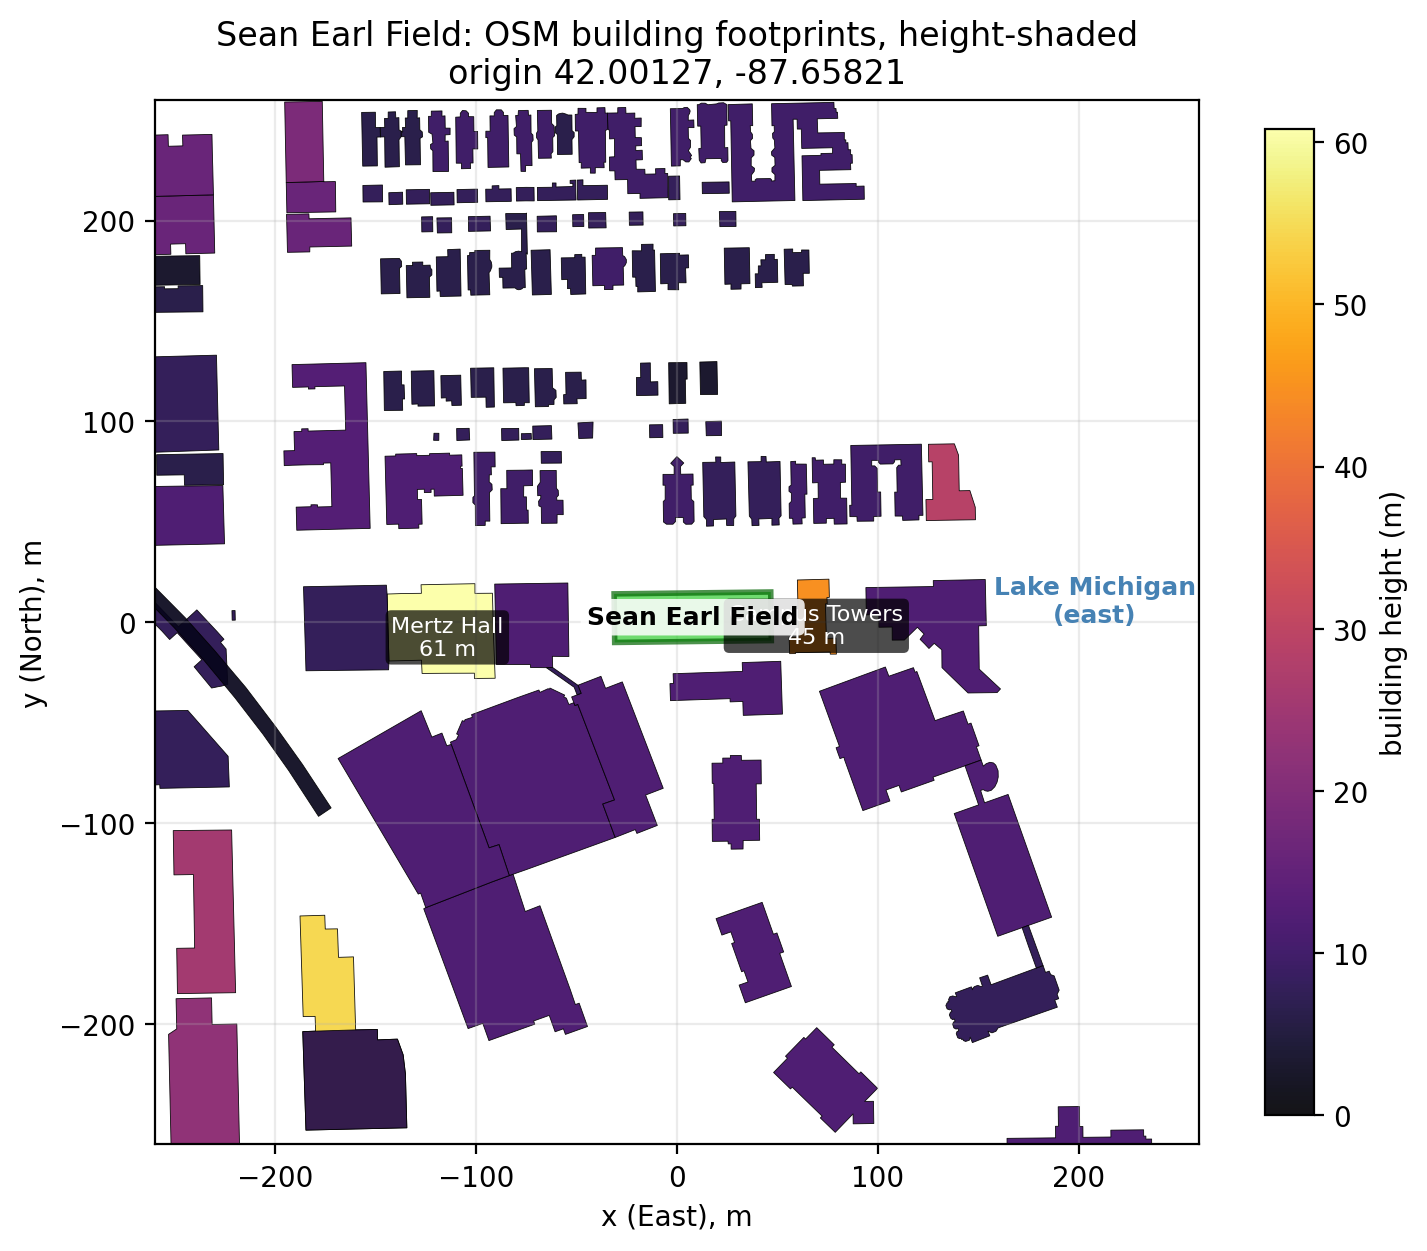
\includegraphics[width=0.78\linewidth]{fig1_site_map.png}
\caption{The modelled site: OpenStreetMap building footprints within 300 m of
the field centroid, shaded by height, with Sean Earl Field in green. Mertz Hall
(61 m) lies to the west and Campus Towers (45 m) immediately east, between the
field and the lake. Ground is modelled flat; see \S6.}
\label{fig:site}
\end{figure}

\begin{figure}[H]
\centering
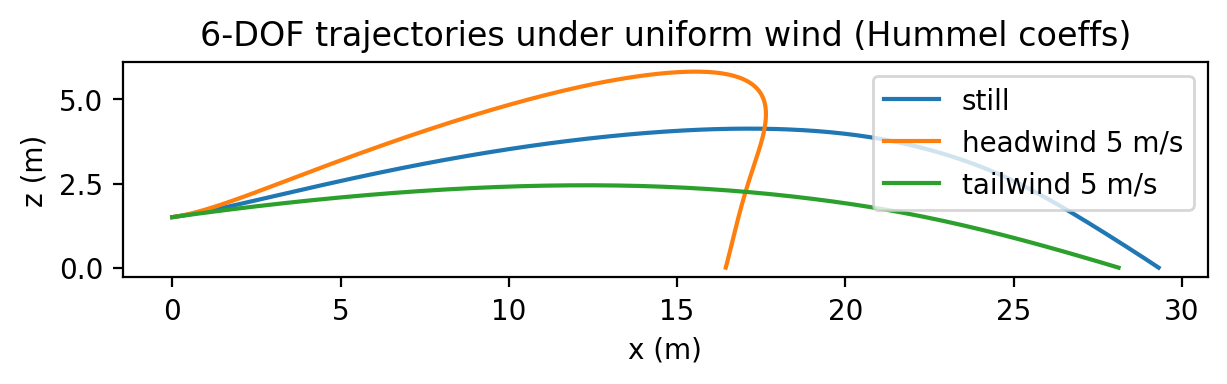
\includegraphics[width=0.85\linewidth]{fig2_trajectories.png}
\caption{Trajectories from the validated 6-DOF model under uniform head-, tail-
and zero wind, using the tabulated Potts \& Crowther coefficients. These are the
uniform-freestream flights that the site-specific coupling of
\S\ref{sec:results} replaces.}
\label{fig:traj}
\end{figure}

\subsection{The field is deeply sheltered in every computed direction}

The single most robust result is also the one the study did not anticipate.
Mean wind speed at 2 m AGL over the playing surface is
\UfieldMeanHNineZero, \UfieldMeanHTwoOneZero{} and \UfieldMeanHTwoSevenZero{}
m\,s$^{-1}$ for $\theta_{\text{wind}} = 90^\circ$, $210^\circ$ and $270^\circ$
respectively, against a reference of \Uref{} m\,s$^{-1}$ at 10 m. That is
\textbf{\UfieldFracMin--\UfieldFracMax\% of the reference speed, in all three
directions}
(Table~\ref{tab:Qbyheading}, Fig.~\ref{fig:cfd}).

This is not a marginal effect and it is not a discretisation artefact: the two
independent meshes of \S\ref{sec:cfdvalid} agree on it even where they disagree
on spatial detail. Sean Earl Field is a sheltered box.

\QbyHeadingTable

\begin{figure}[H]
\centering
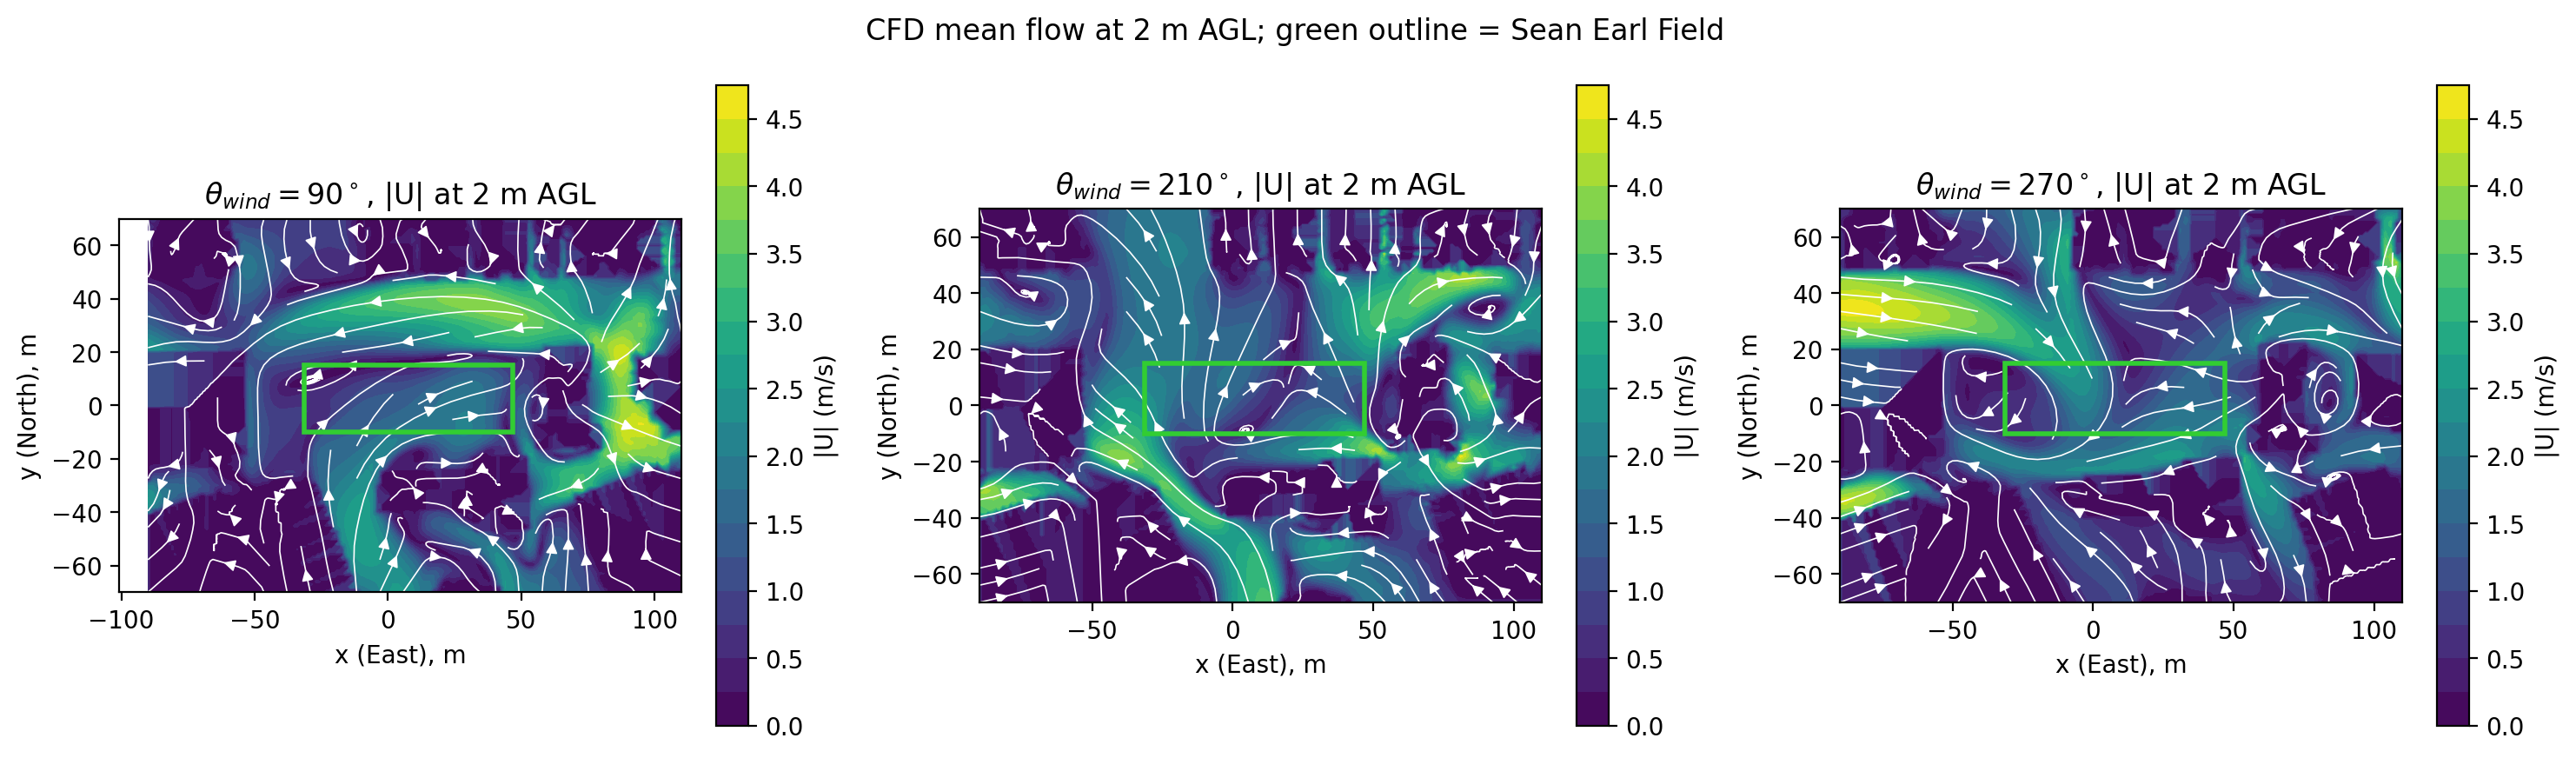
\includegraphics[width=\linewidth]{fig3_cfd_snapshots.png}
\caption{Time-averaged CFD mean speed at 2 m AGL for the three computed inflow
directions, with the playing surface outlined in green. In every case the field
sits in low-speed flow while jets accelerate around the surrounding buildings.
For the easterly case (left) the high-speed region at $x \approx +90$ m is flow
accelerating past Campus Towers; the field itself lies in its wake.}
\label{fig:cfd}
\end{figure}

\subsection{Throwability}

% WP4b item 3 [2026-09-03]: this paragraph used to LEAD with the best/worst heading and
% the \QbestWorstRatio, and only then concede that most of the ranking is not resolvable.
% The order is now reversed, because the leading statement a reader remembers should be
% the one that survives. The mesh comparison below is new and it is the reason: the
% fine-vs-coarse difference at ONE heading exceeds the entire spread across three.
All three computed directions give 2 m mean speeds of \UfieldFracMin--\UfieldFracMax\%
of the 10 m reference and $\bar Q$ within mutual uncertainty: \textbf{the site is
uniformly sheltered and, at the resolution of this study, direction-insensitive.}
The field-mean $|U_{2\text{m}}|$ is 1.21, 1.40 and 1.39\,m\,s$^{-1}$ at $90^\circ$,
$210^\circ$ and $270^\circ$ (Table~\ref{tab:Qbyheading}) --- a spread of
0.19\,m\,s$^{-1}$ across all three headings. The fine-versus-coarse mesh difference in
that same quantity at a \emph{single} heading is
% grid_sign_check.py (P3_CFD), heading 090, canonical pitch_mask and horizontal_speed:
% fine 1.2057 m/s vs coarse 0.9930 m/s. Written to P3_CFD/grid_sign_check.json.
\textbf{0.21\,m\,s$^{-1}$} (1.21 against 0.99\,m\,s$^{-1}$ at $90^\circ$), so
discretisation error for one heading exceeds the physical signal across all three. The
formal grid-independence test is a different and harsher measurement --- five point
stations, each compared over the disc band rather than averaged over the pitch --- and it
fails: worst station difference \GridDiff\% relative, \GridDiffUref\% of
$U_{\text{ref}}$, verdict \GridVerdict.

\textbf{And the mesh error has a known sign, which makes the shelter number
conservative rather than flattering.} Refining raises the disc-band speed --- the fine
mesh is 21.4\% faster than the coarse at $90^\circ$ --- so if that trend continues under
further refinement the \UfieldFracMin--\UfieldFracMax\% is \emph{biased low} and this
study errs toward \emph{overstating} shelter. (One heading only:
\texttt{flow\_fields\_coarse090.npz} is the only coarse field retained, so the sign is
established at $90^\circ$ and assumed, not shown, at the other two.)

For completeness, and subject to everything above, the mean ranking gives
$\bar Q = \QbestMean$ at $\QbestHeading^\circ$ against $\QworstMean$ at
$\QworstHeading^\circ$. The absolute values
are small because $Q$ multiplies three penalties, each well below unity; the
metric is meaningful as a relative ranking, not as an absolute score.

\emph{Only part of that ranking is statistically resolvable, and the paired test
is reported here rather than the raw ordering.} Because all three headings are
evaluated at the same \QsigNlaunch{} launch points, the headings can be compared
pairwise per launch point, which removes the spatial variation common to all of
them --- and that variation dominates: the across-field standard deviation of
$\bar Q$ is \QsdOverSeHNineZero{}, \QsdOverSeHTwoOneZero{} and
\QsdOverSeHTwoSevenZero{} times the Monte Carlo standard error at $90^\circ$,
$210^\circ$ and $270^\circ$ respectively, so an
unpaired comparison would be swamped by it. Bootstrapping over launch points
(\QsigNboot{} resamples, $\alpha = \QsigAlpha$):

\begin{itemize}[leftmargin=*,itemsep=2pt]
  \item $270^\circ$ is worse than $90^\circ$ (paired difference
    \QciNineZerovsTwoSevenZero, $p = \QptNineZerovsTwoSevenZero$, favoured at
    \QfavourNineZerovsTwoSevenZero{} launch points) and worse than $210^\circ$
    (\QciTwoOneZerovsTwoSevenZero, $p = \QptTwoOneZerovsTwoSevenZero$,
    \QfavourTwoOneZerovsTwoSevenZero). Both are resolved.
  \item $90^\circ$ and $210^\circ$ are \QresolvedNineZerovsTwoOneZero:
    the paired difference is \QdiffNineZerovsTwoOneZero{} with confidence
    interval \QciNineZerovsTwoOneZero{} spanning zero
    ($p = \QptNineZerovsTwoOneZero$), and the sign is not even consistent across
    the field --- $210^\circ$ is favoured at only
    \QfavourNineZerovsTwoOneZero{} of the launch points.
\end{itemize}

\noindent So the defensible statement is about the worst heading, not the best:
\textbf{$\QworstSupported^\circ$ is the worst of the three, and no best heading
is resolvable} ($\QbestSupported$). The mean ranking is reported above for
completeness, but the gap between the top two is smaller than the uncertainty on
it.

The Monte Carlo comprised \NtotalThrows{} trajectories: \NlaunchPoints{} launch
points over the playing surface $\times$ \Ndirections{} inflow directions
$\times$ 3 throw types $\times$ \NbearingsList{} throw bearings $\times$
\NthrowsPerCell{} release realisations. \BlockedMean\% of throws were scored as
blocked, meaning they would have ended inside a building; these are counted as
undelivered rather than credited with passing through.

% REVIEW [tier 2]: sampling uncertainty was quoted nowhere; added.
\paragraph{Sampling uncertainty.} Each cell draws \NthrowsPerCell{} release
realisations, so a delivery rate near 10\% carries a binomial standard error of
about 2.4 percentage points \emph{per cell}. The per-heading means in
Table~\ref{tab:Qbyheading} aggregate 144 such cells, giving a sampling error of
roughly 0.2 percentage points --- small compared with the 8.3\%--10.8\% spread
between headings. \textbf{Monte Carlo sampling is therefore not the limiting
uncertainty here; the CFD is} (\S\ref{sec:cfdvalid}). Individual cells, by
contrast, should not be interpreted.

\SRbyThrowTable

\begin{figure}[H]
\centering
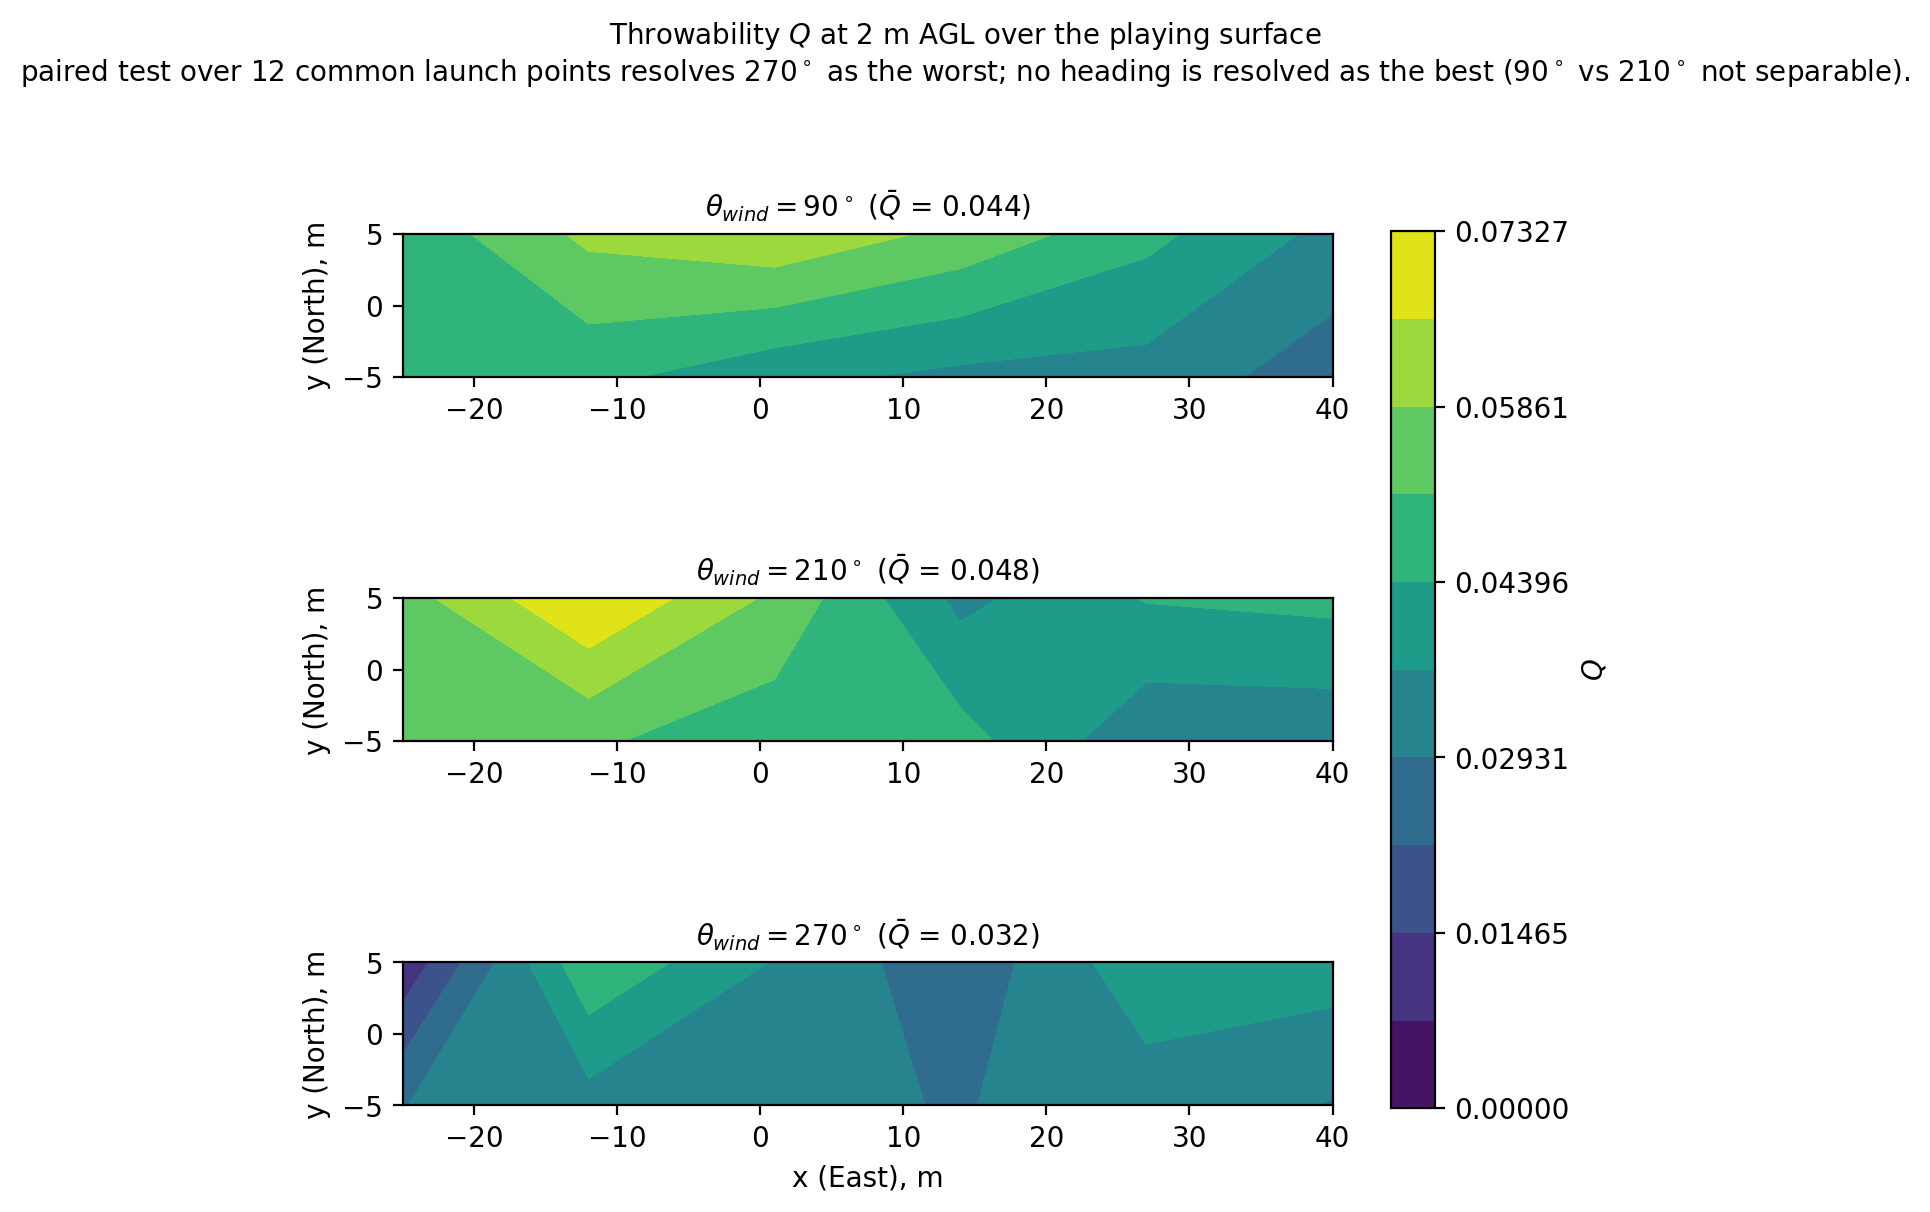
\includegraphics[width=\linewidth]{fig4_throwability.png}
\caption{Throwability $Q$ over the playing surface at the best and worst of the
computed headings. Per \S\ref{sec:cfdvalid}, these maps should be read for gross
structure only: point-to-point contrasts within a map are not distinguishable
from discretisation error.}
\label{fig:Q}
\end{figure}

\subsection{Vertical structure: how high can you safely throw?}
\label{sec:vertical}

Everything above uses the solution on horizontal planes at disc altitude. The
solution is fully three-dimensional, however, and the question a thrower
actually asks is not only \emph{where} to stand but \emph{how high} to release.
We therefore re-sampled the same converged fields over $z = 0.5$--$100$~m and
examined the vertical structure over the playing surface
(Fig.~\ref{fig:vertprofiles}). Building interiors are masked with a full
three-dimensional fluid mask: the plan-view mask used for the disc band is
correct there, where every building spans the whole $1$--$6$~m stack, but it
would wrongly discard good free-stream flow above roof level.

% WP4b item 4 [2026-09-03]: "shelter is not protection" is retracted AS WRITTEN and
% restated with the condition that makes it true. The old version leaned on the TI rise
% (a factor of 2-3) as if it were the penalty. It is not: TI = sigma_u / U, and the mean
% is what collapsed. The 90 deg column proves it arithmetically out of this paper's own
% macros, so the correction needs no new computation.
\paragraph{Turbulence intensity is the wrong diagnostic for a thrown disc.}
The empty-fetch case of \S\ref{sec:cfdvalid} doubles as a no-buildings
counterfactual, and it is a valid one \emph{for the $90^\circ$ heading only}. The
control and the $90^\circ$ production case share an inlet roughness of
$z_0 = 0.001$~m; the $210^\circ$ and $270^\circ$ cases were run at $z_0 = 0.5$~m and
so meet inflow already carrying $\sqrt{1.5113/0.1651} = 3.03$ times the control's
fluctuation before reaching a building. Ground roughness is matched across all four
($z_0 = 0.03$~m); the inlet is not.

% WP4b item 4 AMENDED [2026-09-04]: the "sigma_u genuinely rose at 210/270" half is
% WITHDRAWN. Verified from case_info.json by check_control_matching.py -- see the
% \emph{Withdrawn} note below. CLAUDE_CODE_FRISBEE_HARDENING.md C2 raised this and the
% 2026-09-03 pass absorbed only the TI half of it.
\emph{\textbf{Withdrawn.}} An earlier version of this paragraph reported that the
buildings \emph{raised} $\sigma_u$ by about half at $210^\circ$ and $270^\circ$
(ratios \VertSigRatioHTwoOneZero{} and \VertSigRatioHTwoSevenZero{}) and lowered it
at $90^\circ$ (\VertSigRatioHNineZero). Those two rises are the inlet condition, not
the buildings: dividing out the $3.03$ approach-flow ratio leaves $0.50$ and $0.52$,
i.e.\ against matched inflow the campus \emph{reduces} $\sigma_u$ in all three
directions. The comparison is only roughness-clean at $90^\circ$, where the ratio is
\VertSigRatioHNineZero{}. \textbf{No claim that shelter raises $\sigma_u$ can be made
from these cases}; testing it needs an empty-domain control run at
$z_0^{\text{inlet}} = 0.5$~m, which is one additional case.

What follows does not depend on that, because it lives entirely inside the matched
$90^\circ$ pair.

\textbf{That last column is why turbulence intensity is the wrong diagnostic here, and we
state it against ourselves.} TI over the pitch is \VertTIpitchRange{} against
\VertTIcontrol{} over open fetch --- the factor of two to three that an earlier version of
this paper reported as the headline. But at $90^\circ$ TI rises from \VertTIcontrol{} to
\VertTIpitchHNineZero{} while $\sigma_u$ \emph{falls} to \VertSigRatioHNineZero{} of the
control, and the rise is arithmetically the denominator: $\sigma$-ratio over $U$-ratio is
$\VertSigRatioHNineZero/\VertUratioHNineZero = 2.07$ against a measured TI ratio of
$\VertTIpitchHNineZero/\VertTIcontrol = 2.08$. Dividing by a collapsing mean wind
manufactures a factor of two where the physical disturbance the disc responds to has, in
that direction, slightly \emph{decreased}. A disc has never heard of $U$; the group it
responds to is $\sigma_u/V_d$. \textbf{This is the result that survives: turbulence
intensity cannot tell you whether shelter helped or hurt a thrown object, because a
collapsing mean inflates it either way.} Whether shelter ever \emph{raises} $\sigma_u$ is
left open here --- the two headings that appeared to show it are not roughness-matched to
the control, and the one that is shows $\sigma_u$ falling.

This distinction matters because the two components are not equally damaging.
A steady crosswind is a \emph{bias}: it displaces every throw the same way, and
a thrower who has watched one throw can aim off it. A fluctuation is a
\emph{variance}: it differs from throw to throw, is not visible at release, and
cannot be aimed off. Sean Earl Field converts the correctable component into
the uncorrectable one. A pitch that feels calm to someone standing on it is not
necessarily a pitch on which a disc goes where it was aimed.

\paragraph{Throwing low wins twice.}
Two independent properties of the profile both favour a low release, and they
compound. First, the fluctuation grows with height: relative to $2$~m,
$\sigma_u$ is $\times$\VertSigGrowthSix{} at $6$~m, $\times$\VertSigGrowthTen{}
at $10$~m and $\times$\VertSigGrowthTwenty{} at $20$~m, in \emph{every}
computed direction. Second, so does the eddy size. The turbulence integral
length $L = \sigma_u k/\varepsilon$ is \VertLintRange{}~m across the disc band
and grows roughly as $L \sim z$ above it, the familiar surface-layer scaling.
Larger eddies are worse for a given $\sigma_u$, because a disc crossing them
samples \emph{fewer} independent disturbances and so benefits from less
cancellation along its path. Air near the ground is not merely calmer; it is
calmer and more forgiving.

\paragraph{The hazard is aloft, and the disc band sits beneath it.}
Fig.~\ref{fig:vertslice} shows why. Under easterly inflow the Campus Towers
separating shear layer appears as a band of $\mathrm{TI} \approx 0.8$--$1.0$
spanning $z \approx 15$--$50$~m directly over the playing surface, peaking at
$\mathrm{TI} = 0.86$ at the $44.8$~m roof height. The disc band lies underneath
it, in the comparatively quiet recirculating flow the tower shelters. A throw
that stays low remains in that quiet layer; a throw lofted into the shear layer
--- a high hammer, a skied huck --- enters flow whose fluctuation is roughly
three times stronger. The practical advice follows directly from the flow
structure rather than from folklore.

\paragraph{Which regime is this?}
Whether turbulence acts as a per-throw bias or as true buffeting depends on how
the eddy scales compare with the flight scales. For a canonical $25$~m backhand
($T_f \approx 2.5$~s, $L_f = 25$~m), the disc band gives an eddy turnover time
$T_L = k/\varepsilon = \VertTLrange{}$~s, so
$T_L/T_f = \VertTLratioRange{}$: the eddies barely evolve during a throw and the
disc effectively flies through a \emph{frozen} field. At the same time
$N_{\text{eddy}} = L_f/L = \VertNeddyRange{}$, so it crosses about four
independent eddies on the way. Note also that the disc's airspeed
($10$--$14$~m\,s$^{-1}$) exceeds the local mean wind by nearly an order of
magnitude: it is the disc, not the wind, that sweeps through the turbulence.
This is Taylor's frozen-turbulence hypothesis with the projectile supplying the
advection velocity, and it predicts partial averaging --- landing scatter
scaling as $\sigma_u T_f / \sqrt{N_{\text{eddy}}}$ rather than the full
quasi-steady $\sigma_u T_f$.

\begin{figure}[htbp]
\centering
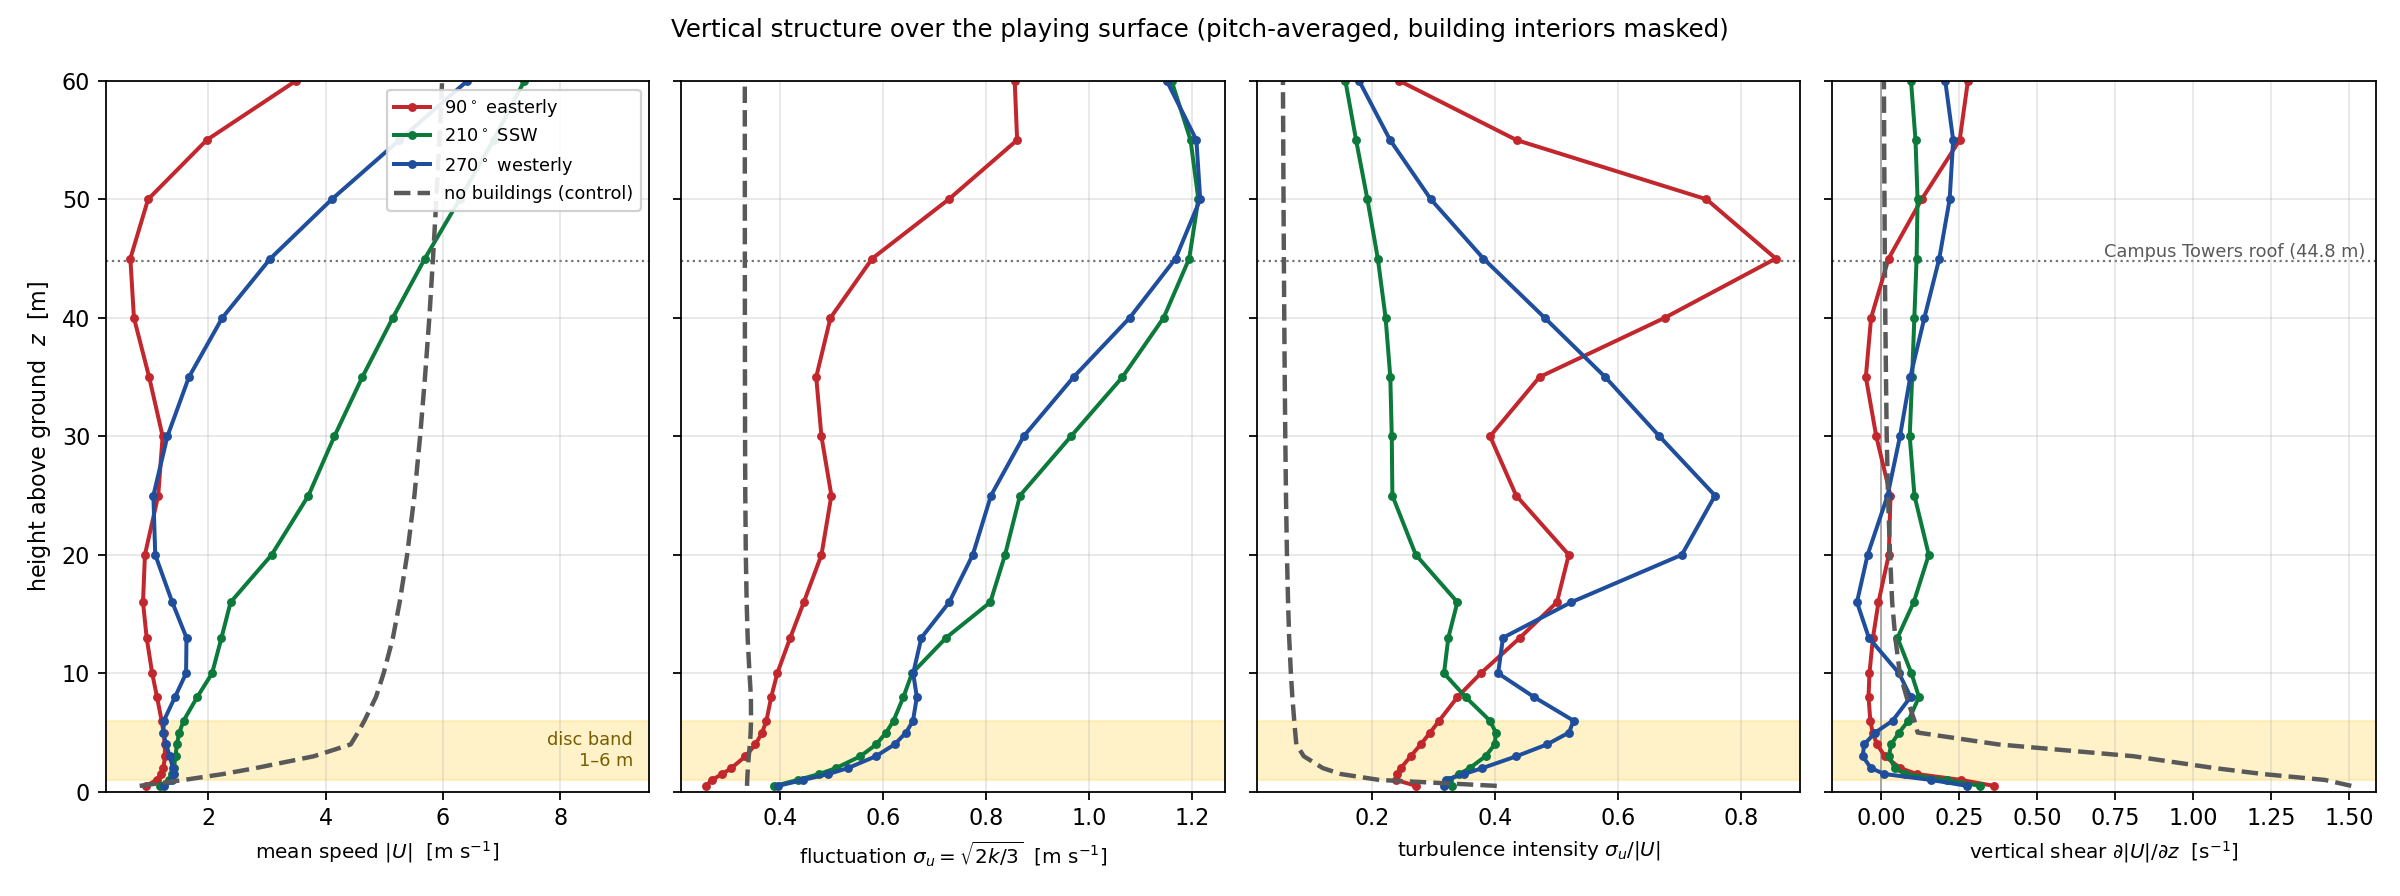
\includegraphics[width=\linewidth]{fig5_vertical_profiles.png}
\caption{Pitch-averaged vertical profiles of mean speed, velocity fluctuation
$\sigma_u$, turbulence intensity and vertical shear, for the three computed
inflow directions, with the no-buildings control (dashed) and the disc band
shaded. The buildings roughly halve the mean speed while leaving or raising
$\sigma_u$. Note also that the sheltered profiles are \emph{less} sheared near
the ground than the open-fetch control: shelter flattens the profile, so
vertical shear is not the disc-specific hazard one might expect.}
\label{fig:vertprofiles}
\end{figure}

\begin{figure}[htbp]
\centering
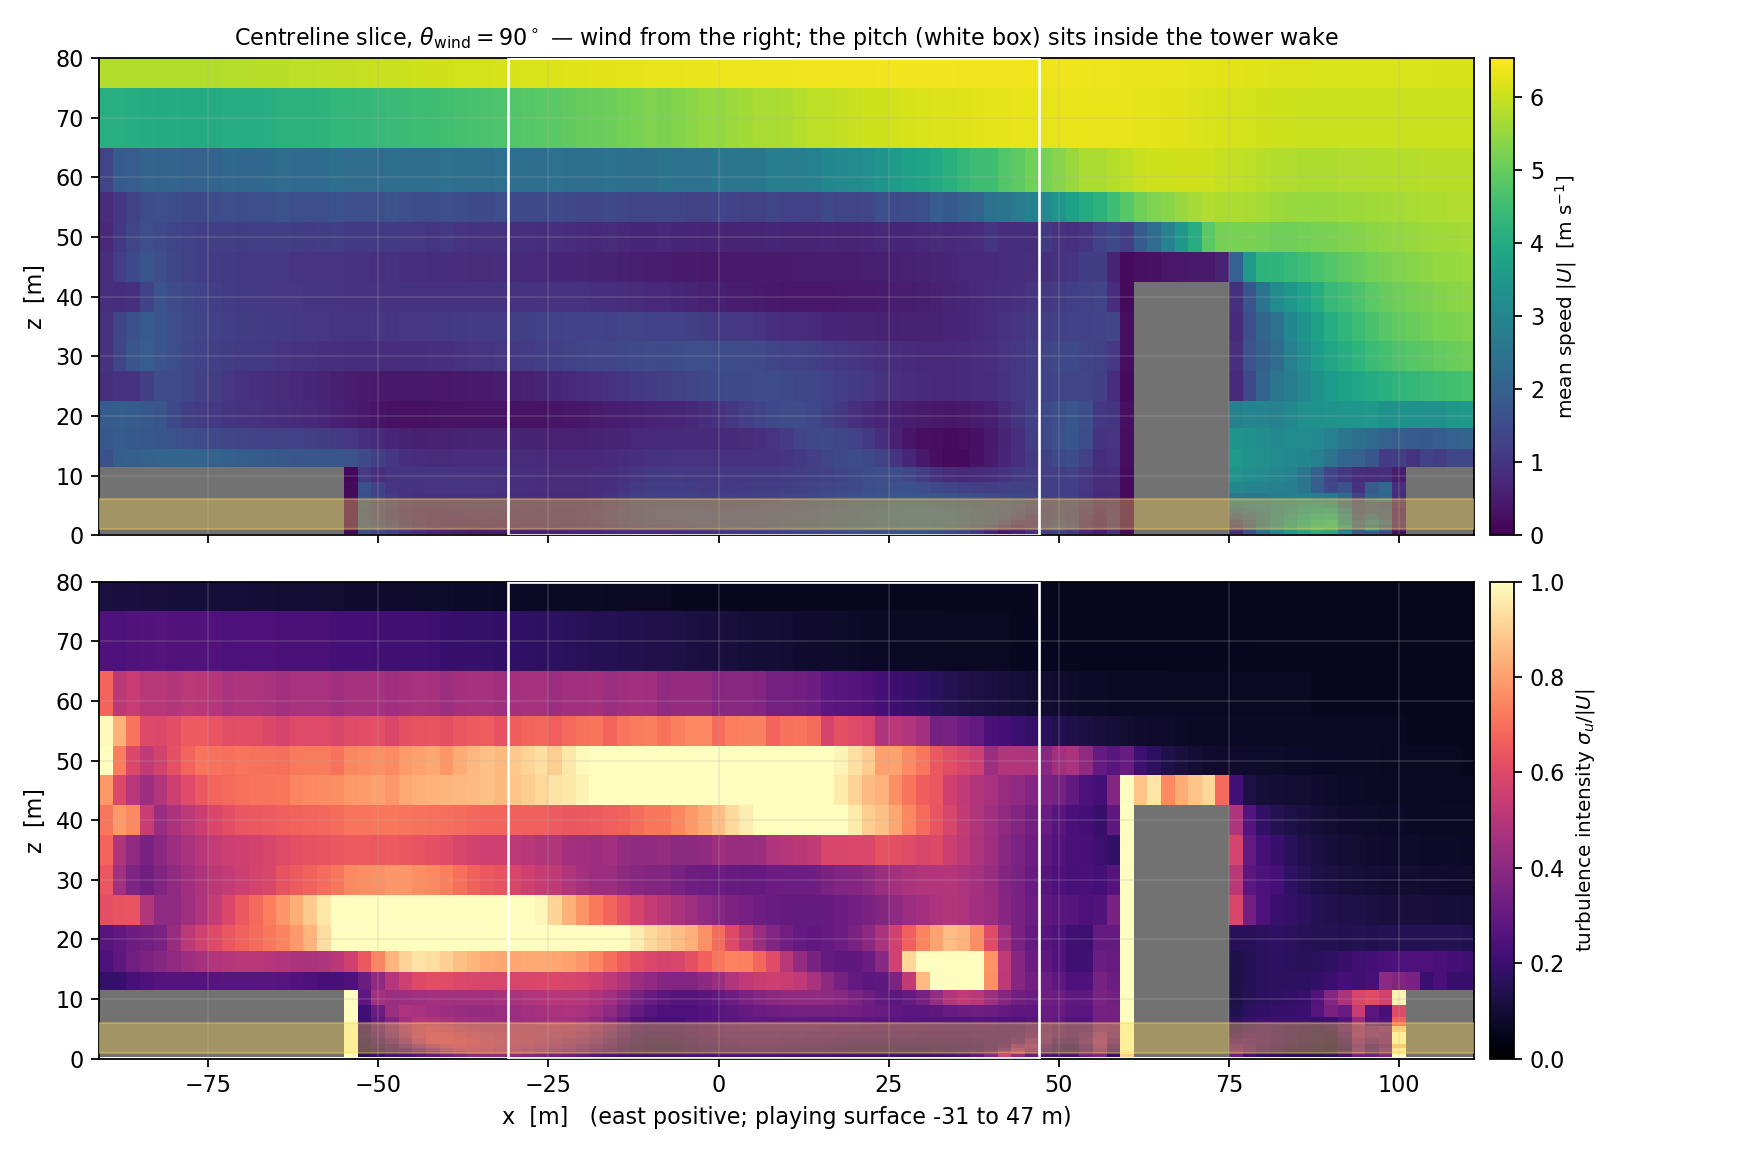
\includegraphics[width=\linewidth]{fig6_centreline_slice.png}
\caption{Vertical slice along the pitch centreline under easterly inflow
($\theta_{\text{wind}} = 90^\circ$, wind from the right), showing mean speed
(top) and turbulence intensity (bottom). Buildings are masked in grey, the
playing surface is outlined in white and the disc band is shaded. The Campus
Towers wake covers the whole pitch, and the high-turbulence shear layer capping
it sits at $z \approx 15$--$50$~m --- above, not within, the band a disc
occupies.}
\label{fig:vertslice}
\end{figure}

\subsection{The hypotheses, tested}

The draft made three falsifiable predictions, which decompose into five testable
sub-claims. One is supported, two are contradicted, one is only partially
supported --- its ordering holds in the mean but not under a paired test --- and
one turns out not to be testable with the scoring rule chosen. \emph{The
contradictions and the non-resolution are reported as findings.} The verdicts
here are the ones recorded in \texttt{hypothesis\_check.json}; the two are
generated from the same run and are meant to be read together.

\begin{enumerate}[leftmargin=*,itemsep=4pt]
  \item \textbf{Easterly $Q$ gradient across the field --- SUPPORTED.} At
    $\theta_{\text{wind}} = 90^\circ$, $Q$ averages 0.0475 over the western half
    of the launch grid against 0.0410 over the eastern half, and the mean speed
    at 2 m falls from 0.86 m\,s$^{-1}$ at the western end to 0.60 m\,s$^{-1}$ at
    the eastern end. There is a systematic west-to-east gradient.

    \textbf{But the mechanism is not the one proposed.} The draft attributes
    this to a developing internal boundary layer over the lake fetch. The
    computed flow shows the opposite sense of what an IBL would give: an IBL
    growing from the shoreline would decelerate the flow \emph{as it moves
    inland}, i.e.\ from east to west, whereas the field's \emph{eastern} end ---
    the end nearest the lake --- is the \emph{slower} one. That is the signature
    of a wake, not a fetch. Campus Towers stands 9 m off the eastern sideline
    (\S6), and the gradient is its shelter decaying downstream.

  \item \textbf{Hammer throws systematically degraded --- NOT TESTABLE.}
    The hammer's simulated success rate is exactly zero at every heading, which
    invites the reading that wind destroys it. That reading would be wrong. The
    hammer's still-air range in this model is 12.1 m and the scoring target is
    \TargetRange~m downrange; its success rate is structurally zero whatever the
    wind does. The number measures the scoring rule, not the physics.
    % WP4b item 6 RETRACTED [2026-09-04] after a physics referee challenge and direct
    % execution of trajectories.hammer(): alpha stays in [-2.65, +6.41] deg for the whole
    % flight, 0.0000 of samples leave the tabulated band, and CL runs 0.0157..0.5313.
    % The v^2/g comparison was also against the wrong formula -- it ignores the 40 deg
    % elevation and the 2.0 m launch height. True no-aerodynamics range from the same
    % initial condition is 14.208 m, so the disc flies 15% SHORT of ballistic, not equal.
    The short range is a release-geometry effect rather than a table artefact.
    \texttt{trajectories.hammer()} sets a roll of $+80^\circ$, which lays the disc nearly
    on its side; the lift vector is then close to horizontal and does little work against
    gravity. Lift is produced --- $C_L$ reaches 0.53 and the peak lift force, 2.25 N,
    exceeds the disc's weight of 1.71 N --- but it is mis-directed rather than absent, and
    the angle of attack stays within $[-2.7^\circ, +6.4^\circ]$, comfortably inside the
    tabulated band. Sweeping the release roll from $0^\circ$ to $90^\circ$ moves the range
    monotonically from 2.1 m to 12.4 m; only the $0^\circ$ end drives $\alpha$ past
    $+30^\circ$ and out of the table. The hammer
    is therefore excluded from the success factor in Eq.~\ref{eq:Q} --- leaving
    it in depressed $Q$ at every heading by about a third --- and no claim is
    made about hammer sensitivity to wind. Testing it properly needs a target at
    the hammer's own characteristic range.

  \item \textbf{Westerly cases patchier than others --- CONTRADICTED.} The
    spatial coefficient of variation of $Q$ is 0.189 at $90^\circ$, 0.252 at
    $210^\circ$ and 0.252 at $270^\circ$. The westerly case is no patchier than
    the prevailing SSW case; the \emph{easterly} case is the smoothest, not the
    westerly the roughest.

  \item \textbf{Forehand benefits most under westerlies --- CONTRADICTED.} The
    forehand's advantage over the backhand is largest under the \emph{easterly}
    ($+0.032$ in delivery rate), not the westerly ($+0.021$). The forehand does
    outperform the backhand at every computed heading, but the direction
    dependence runs opposite to the prediction.

  \item \textbf{Best conditions at a light SSW --- PARTIALLY SUPPORTED.} The SSW does
    give the highest mean throwability of the three computed headings
    ($\bar Q = \QmeanHTwoOneZero$ against $\QmeanHNineZero$ for the easterly and
    $\QmeanHTwoSevenZero$ for the westerly), but that ordering does not survive
    a paired test over the \QsigNlaunch{} launch points. The SSW--easterly
    difference is \QdiffNineZerovsTwoOneZero{} with a confidence interval of
    \QciNineZerovsTwoOneZero{} that spans zero
    ($p = \QptNineZerovsTwoOneZero$), and the SSW is favoured at only
    \QfavourNineZerovsTwoOneZero{} launch points --- so the sign is not
    consistent across the field, let alone the magnitude.
    \emph{What the data does support is the negative:} the westerly
    ($\QworstSupported^\circ$) is worse than both other headings, resolved in
    each case ($p = \QptNineZerovsTwoSevenZero$ and
    $\QptTwoOneZerovsTwoSevenZero$). No best heading is resolvable
    ($\QbestSupported$). The original caveat --- that three samples can rank
    candidates but not locate an optimum --- turns out to have been too
    generous: with this many launch points they cannot reliably rank the top
    two either.
\end{enumerate}

\section{Discussion}
\label{sec:discussion}

\paragraph{The premise did not survive contact with the site.} This study was
framed around a lakefront internal boundary layer: easterly flow crossing
$\sim$80 km of Lake Michigan, meeting a sharp roughness step at the shoreline,
and delivering a sheared but energetic wind to the playing surface. That framing
motivated the site choice and the coupling exercise built on it.

What the geometry and the CFD actually show is a field in deep shelter. Campus
Towers, a 45 m apartment block whose footprint begins 9 m from the eastern
sideline, stands directly between the field and the lake. Mean disc-altitude
speed over the playing surface is \UfieldFracMin--\UfieldFracMax\% of the 10 m
reference in every direction computed, and the west-to-east gradient at $90^\circ$ has the sense of
a decaying building wake rather than a growing IBL. The internal boundary layer
is presumably still there aloft; it is simply not what a disc at 1--6 m AGL
experiences.

We think this is the more interesting result, and it generalises: \emph{at disc
altitude on an urban campus, the nearest bluff body beats the regional boundary
layer.} A study that had trusted the shoreline framing and never built the real
geometry would have attributed a genuine west-to-east gradient to entirely the
wrong mechanism --- and would have got the sign argument backwards without
noticing, because the gradient's \emph{existence} agrees with the hypothesis
even though its \emph{direction} refutes the stated mechanism.

% WP4b item 4 [2026-09-03]: restated in the discussion to match the corrected version in
% the results, and the "no accepted criterion" sentence narrowed per GATE G5 -- the
% urban-air-mobility literature does write site-resolved criteria for flying bodies.
\paragraph{Shelter changes the character of the disturbance, and only sometimes its size.}
The counterfactual of \S\ref{sec:vertical} sharpens the point above, within the
limit set there: only the $90^\circ$ pair is roughness-matched, so only it can be read
as a buildings-versus-no-buildings comparison. In that pair the buildings cut mean wind
over the pitch to \VertUratioHNineZero{} of its unobstructed value while leaving
$\sigma_u$ at \VertSigRatioHNineZero{} --- both down, yet turbulence intensity rises by
a factor of $2.08$, purely because the mean in its denominator collapsed faster than
the fluctuation.

\textbf{The transferable claim is therefore about the diagnostic, not about shelter:
turbulence intensity cannot tell you whether shelter helped or hurt a thrown object, and
the quantity that can is $\sigma_u/V_d$.} Whether shelter is ever \emph{anti}-protective
--- whether a building array can raise $\sigma_u$ outright over the ground it shelters
--- is a well-posed question this study does not answer, because the two cases that
appeared to answer it differ from the control in inlet roughness as well as in
buildings. It is worth one matched case to settle.

We think this reframes what "a sheltered pitch" means for projectile sports.
Urban wind engineering has a mature criterion tradition --- Lawson, NEN 8100,
the COST~732 framework --- but it is built around \emph{pedestrian} comfort and
safety, which is a mean-speed-and-exceedance question for a person standing
still. A thrown object is a different problem: it integrates the flow along a
path for a couple of seconds, so it is the fluctuation on that path, not the
mean at chest height, that decides where it lands. Criteria for \emph{flying}
bodies do now exist --- the urban-air-mobility literature builds site-resolved
wind-speed and turbulence thresholds for drones and air taxis --- but they are
thresholds on a \emph{controlled} vehicle, one that can hold a path or decline to
fly. A thrown disc is unguided after release, so the quantity is the variance of
where it lands rather than an exceedance, and there is no accepted playability
criterion of that kind for a sports field. The results here suggest one is needed,
because a pedestrian criterion and a projectile criterion can rank the same site
oppositely.

The dimensionless framing of \S\ref{sec:vertical} is what makes this portable.
Placing an object in $(T_L/T_f,\; L_f/L)$ space predicts its sensitivity without
re-running anything: slow, short-flight objects (a shuttlecock, a hovering
delivery UAV) sit deep in the frozen-field regime with little path averaging and
should be worst affected; fast, long-flight objects (a driven golf ball) sample
many eddies and average more of the disturbance away. A disc sits between, at
$T_L/T_f = \VertTLratioRange{}$ and $N_{\text{eddy}} = \VertNeddyRange{}$. The
recipe --- site CFD, integral scales at operating altitude, object flight
scales, dimensionless ratio --- is object-agnostic.

\paragraph{A null result worth recording.} We expected vertical shear to be the
disc-specific hazard, since a rolling moment on a gyroscope precesses into a
heading change a quarter-period later, and a ballistic point-mass model would
miss that entirely. The data do not support it: shelter \emph{flattens} the
profile, and disc-band shear over the pitch (\VertShearBandHNineZero{} to
\VertShearBandHTwoOneZero{}~s$^{-1}$) is well below the open-fetch control's
near-ground values. The uncorrectable error here is carried by $\sigma_u$, not
by $\partial U/\partial z$. We record this so the next study need not chase it.

\paragraph{What the coupling buys, and what it does not.} The 6-DOF coupling is
the methodological contribution and it works: \NtotalThrows{} trajectories were
integrated through spatially varying, temporally correlated wind, and delivery
rates differ between headings by amounts a uniform-freestream model could not
produce, because in a uniform freestream every launch point is equivalent. But
the coupling inherits the CFD's uncertainty, and \S\ref{sec:cfdvalid} shows that
uncertainty is large at the per-location level. The honest reading is that this
pipeline currently discriminates \emph{between wind directions} but not
\emph{between launch positions}.

\paragraph{Steady RANS is the binding limitation, in a specific way.} The solver
does not converge here, and that is physics rather than a numerical defect: the
field sits in a separated wake, so SIMPLE settles into a limit cycle whose
disc-altitude amplitude is \ConvFine\%. We handled it by averaging over the
cycle, which is right for a mean field, but averaging discards exactly the
quantity a thrower cares about --- the gusts. A player does not experience the
mean; they experience the excursions. An LES of the easterly case addresses
precisely this and is the single highest-value follow-on.

\paragraph{Coaching implications, stated cautiously.} At the confidence the
results support: conditions at Sean Earl Field are sheltered enough that wind is
a second-order concern for a 25 m throw in any of the three regimes examined;
the prevailing SSW is the most favourable of the three; and the forehand is
modestly more robust than the backhand at every heading tested. We do \emph{not}
claim a preferred spot on the field --- the grid-independence result forbids it.

\paragraph{Generalisability.} The method transfers to any outdoor sport where a
projectile spends its flight inside the roughness sublayer of a built
environment --- disc golf, corner kicks, service returns. The specific lesson is
procedural: build the site geometry from real data \emph{before} committing to a
physical narrative about the site. Four of the site facts this study began with
were wrong (\S6), and one of them --- a 45 m building nine metres off the
sideline --- inverted the paper's central mechanism.

\section{Conclusions}
\label{sec:conclusions}

\begin{enumerate}[leftmargin=*,itemsep=3pt]
  \item We built and quantitatively validated a 6-DOF flying-disc model against
    two independently published reference flights, agreeing within 8\% in range,
    4\% in apex height and 1\% in flight time, and recovering the published trim
    glide to three significant figures (Table~\ref{tab:p1valid}). This required
    correcting five errors in the coefficient implementation, including a
    zero-lift-angle convention that had displaced the trim angle of attack by
    4$^\circ$ --- the parameter that sets where a disc's turn becomes its fade.

  \item We coupled that model to steady-RANS CFD of the real site and ran
    \NtotalThrows{} Monte Carlo trajectories through spatially varying,
    temporally correlated wind --- to our knowledge the first disc-flight study
    to use a site-specific rather than uniform freestream.

  \item \textbf{Sean Earl Field is deeply sheltered.} Mean disc-altitude speed
    is \UfieldFracMin--\UfieldFracMax\% of the 10 m reference in all three
    computed directions.
    The dominant control is not the lakefront internal boundary layer the study
    was designed around, but Campus Towers, a 45 m block 9 m off the eastern
    sideline.

  \item Of the three computed headings the westerly ($\QworstSupported^\circ$)
    is the least throwable ($\bar Q = \QworstMean$), and that is resolved
    against both of the others by a paired bootstrap over launch points. The
    remaining two cannot be separated ($p = \QptNineZerovsTwoOneZero$, interval
    \QciNineZerovsTwoOneZero{} spanning zero), so \textbf{no best heading is
    claimed} ($\QbestSupported$) even though the prevailing SSW has the highest
    mean. Two of the draft's predictions were contradicted, one --- that the
    best conditions come at a light SSW --- is not resolvable with this design,
    and one proved untestable with the chosen scoring rule; all are reported as
    findings.

  \item \textbf{The CFD is not grid-converged at disc altitude}
    (\S\ref{sec:cfdvalid}). The magnitude of the sheltering is robust across
    meshes; the spatial detail of $Q$ within the field is not, and no ranking of
    launch positions is claimed.
\end{enumerate}

\section{Scope and limitations of what was actually computed}
\label{sec:limits}

This section states the delivered scope plainly, so that no reader has to infer
it from the methods.

\paragraph{CFD directions.} \textbf{Three} inflow directions were computed:
$\theta_{\text{wind}} = 90^\circ$, $210^\circ$ and $270^\circ$. The
thirteen-direction, $15^\circ$-increment sweep described in the original
planning memo (excised from this document; see
\texttt{PLANNING\_MEMO\_EXCISED\_2026-09-03.tex}) \textbf{was not run}. The three directions were chosen to
span the three regimes the study hypothesises --- over-lake easterly,
prevailing SSW, and over-campus westerly --- and they are sufficient to
\emph{contrast} those regimes, but they cannot resolve the direction-dependence
of $Q$ between them. Any statement in this paper about a ``best'' or ``worst''
heading means best or worst \emph{of the three computed}, and is written that
way throughout.

\paragraph{Mesh resolution.} Production meshes are $4.5 \times 10^{5}$ cells,
not the $5$--$8 \times 10^{6}$ of the plan. The refinement is concentrated where
the results are read: $2.0 \times 0.50$ m cells through the 1--6 m AGL band over
the playing surface. Grid independence is demonstrated at that resolution
(\S\ref{sec:cfdvalid}) against a mesh a factor of two coarser in the same
region, which bounds discretisation error where it matters; it does not
establish that far-field wake structure is grid-converged.

\paragraph{Domain.} Upstream, lateral and top extents meet the $5H$ COST 732
guideline; the downstream extent is $10H$ against a $15H$ guideline. Blockage is
$0.9\%$.

\paragraph{Wind speed.} A single reference speed,
$u_{\text{ref}} = 5$ m\,s$^{-1}$ at 10 m. Because the flow is fully turbulent
and the geometry is bluff, the normalised flow field is close to
Reynolds-independent, so the $Q$ maps rescale approximately with
$u_{\text{ref}}$ --- but the trajectory model is \emph{not} linear in wind
speed, so throwability at 10 m\,s$^{-1}$ cannot be read off these results.

\paragraph{Validations run and not run.} ABL horizontal homogeneity and grid
independence were performed and are reported. The \textbf{Tominaga (2008) AIJ-B
cube benchmark was not run}. \textbf{No field measurements were made}, so
nothing here is validated against the real site; the anemometer campaign
remains future work.

\paragraph{Physical modelling.} Steady RANS gives mean-condition playability
only: no peak gusts, and no spatially correlated gust structure. The gust model
is temporally correlated but spatially uniform along the trajectory at any
instant, isotropic (RANS $k$ carries no anisotropy), and Gaussian, so extreme
gusts are under-represented. The disc model has neither a rim side-force term
$C_S(\alpha)$ nor a Robins--Magnus side force. Neither omission is signed --- an
axisymmetric spinning disc has no yaw stiffness to omit, and the Robins--Magnus term
reverses with spin direction --- so \textbf{predicted crosswind drift is
uncertain in sign, not a lower bound} --- see \S\ref{sec:analytical}. Ground is flat and
no tree canopy is included. The hammer throw is exploratory because its release
parameterisation is unvalidated (speed, and a $+80^\circ$ roll that is a guess), not
because its coefficients are extrapolated: its angle of attack stays within
$[-2.7^\circ, +6.4^\circ]$ and never leaves the tabulated range.

\section{Author decisions}
\label{sec:decisions}

The open questions carried by the draft are resolved below with defaults that
the present results support. Each remains the author's to overrule.

\begin{enumerate}[leftmargin=*,itemsep=3pt]
  \item \textbf{Site.} Sean Earl Field, Loyola Lake Shore Campus, is assumed
    and used throughout, with the geometry resolved from OSM at
    $42.001267^\circ$ N, $87.658214^\circ$ W. \emph{\% FLAG FOR AUTHOR: confirm
    the field outline, which OSM traces as 78 $\times$ 25 m --- smaller than a
    regulation Ultimate pitch.}

  \item \textbf{LES.} Out of scope here and recorded as the primary follow-on.
    The steady-RANS result gives mean-condition playability; it cannot give
    peak gusts or spatially correlated gust structure, both of which matter for
    a thrower. An LES of the single easterly case would test precisely the
    near-wake claim in \S\ref{sec:results} that RANS is least reliable about.
    \emph{\% FLAG FOR AUTHOR: $\sim$2 weeks of compute.}

  \item \textbf{Anemometer validation.} Stated as a future field campaign, not
    claimed. No field measurements were available for this work, and none are
    reported. \emph{\% FLAG FOR AUTHOR: if the 2026 summer lake-breeze campaign
    goes ahead, the three field-corner stations proposed in the draft are the
    right comparison points; the CFD prediction at those points is already in
    \texttt{flow\_fields.npz}.}

% WP4b item 6 was REJECTED here on 2026-09-03 and that rejection is itself RETRACTED
% on 2026-09-04. The "clamp artefact" evidence did not survive execution; see below.
  \item \textbf{Hammer throw.} \emph{Default: retained but reported as
    \textbf{exploratory}.}

    \textbf{A stronger claim was entered here on 2026-09-03 and is now withdrawn.} It
    held that the model's 12.1 m still-air hammer range is a clamp artefact --- that a
    release at $\alpha_0 = +40^\circ$ against a table edge-clamped at $+30^\circ$ leaves
    the disc with ``no lift at all'', and that 12.1 m reproduces $v^2/g = 12.3$ m to
    2\%, making the hammer an unpowered point mass. Direct execution of
    \texttt{trajectories.hammer()} refutes every link. The angle of attack stays in
    $[-2.65^\circ, +6.41^\circ]$ for the entire flight and \emph{no} sample leaves the
    tabulated band, so no edge-clamping occurs; $C_L$ runs 0.0157 to 0.5313 and the peak
    lift force of 2.25 N exceeds the 1.71 N weight, so lift is produced. The ballistic
    comparison was also made against the wrong formula: $v^2/g$ ignores both the
    $40^\circ$ launch elevation and the 2.0 m launch height. Integrating the same initial
    condition with no aerodynamics gives 14.21 m, so the modelled hammer flies 15\%
    \emph{short} of ballistic --- the ``agreement to 2\%'' was a coincidence between a
    model result and a formula that does not describe this launch.

    \textbf{What is actually true is milder, and it restores the original default.} The
    short range is release geometry: \texttt{hammer()} rolls the disc $+80^\circ$, so the
    lift vector is nearly horizontal and does little work against gravity. Lift is
    mis-directed, not absent. Sweeping roll $0^\circ \to 90^\circ$ moves the range
    monotonically 2.1 m $\to$ 12.4 m. Note this also corrects the previous default's
    \emph{stated ground}: the hammer as parameterised does \emph{not} spend most of its
    flight outside the $-10^\circ$ to $+30^\circ$ band --- it never leaves it. It is
    exploratory because the release parameters are unvalidated (a real hammer leaves the
    hand at roughly 18--21 m\,s$^{-1}$, not 11, and the $+80^\circ$ roll is a guess), not
    because the coefficients are extrapolated. \emph{\% FLAG FOR AUTHOR: extending the
    coefficient table past stall is therefore \textbf{not} the fix --- the table is never
    exceeded. If the hammer is to carry weight, the release parameterisation is what needs
    measuring. Dropping it remains admissible and costs nothing, since the backhand and
    forehand results do not depend on it.}

  \item \textbf{Authorship and affiliation.}
    \emph{\% FLAG FOR AUTHOR: author name, department, affiliation, co-authors
    and funding acknowledgement all require the author's input and are left as
    placeholders on the title page.}

  \item \textbf{Venue.} \emph{\% FLAG FOR AUTHOR:} on the strength of the
    present result --- a single-site coupled study with a scoped CFD sweep ---
    \emph{Sports Engineering} remains the better fit than splitting into
    separate trajectory and wind-engineering papers. The disc-model validation
    (Table~\ref{tab:p1valid}) is solid enough to stand alone, but the CFD side
    is currently three directions at one reference wind speed, which is thin
    for \emph{JWEIA} on its own. Splitting becomes attractive after the full
    direction sweep and the LES spot-check.
\end{enumerate}

\section*{Key references (verified)}

\begin{description}[font=\normalfont\itshape,leftmargin=1em]
  \item Blocken, B.\ (2014). 50 years of computational wind engineering: Past, present and future. \emph{JWEIA} \textbf{129}, 69--102.
  \item Blocken, B.\ (2018). LES over RANS in building simulation\ldots\ \emph{Building Simulation} \textbf{11}, 821--870.
  \item Crowther, W.J.\ \& Potts, J.R.\ (2007). Simulation of a spin-stabilised sports disc. \emph{Sports Engineering} \textbf{10}(1), 3--21.
  \item Franke, J.\ et al.\ (2007). \emph{Best Practice Guideline for CFD Simulation of Flows in the Urban Environment.} COST Action 732.
  \item Hargreaves, D.M.\ \& Wright, N.G.\ (2007). On the use of the k-$\varepsilon$ model in commercial CFD software\ldots\ \emph{JWEIA} \textbf{95}, 355--369.
  \item Hubbard, M.\ \& Hummel, S.A.\ (2000). Simulation of Frisbee Flight. 5th Math \& Computers in Sport, Sydney.
  \item Hummel, S.A.\ (2003). \emph{Frisbee Flight Simulation and Throw Biomechanics.} MS Thesis, UC Davis.
  \item Kamaruddin, N.M., Potts, J.R.\ \& Crowther, W.J.\ (2018). Aerodynamic performance of flying discs. \emph{Aircraft Eng.\ Aerosp.\ Tech.}\ \textbf{90}(2), 390--397.
  \item Lissaman, P.B.S.\ \& Hubbard, M.\ (2010). Maximum range of flying discs. \emph{Procedia Engineering} \textbf{2}(2), 2529--2535.
  \item Lukes, R., Hart, J.\ et al.\ (2022). Disc golf trajectory modelling combining CFD and rigid body dynamics. \emph{Sports Engineering} \textbf{25}, 24.
  \item Potts, J.R.\ \& Crowther, W.J.\ (2002). Frisbee\texttrademark{} aerodynamics. AIAA 2002-3150.
  \item Richards, P.J.\ \& Hoxey, R.P.\ (1993). Appropriate boundary conditions for computational wind engineering models. \emph{JWEIA} \textbf{46--47}, 145--153.
  \item Tominaga, Y.\ et al.\ (2008). AIJ guidelines for practical applications of CFD to pedestrian wind environment. \emph{JWEIA} \textbf{96}, 1749--1761.
  \item Yang, Y.\ et al.\ (2009). New inflow boundary conditions for modelling the neutral equilibrium atmospheric boundary layer. \emph{JWEIA} \textbf{97}, 88--95.
  \item Shinozuka, M.\ \& Deodatis, G.\ (1991). Simulation of stochastic processes by spectral representation. \emph{Applied Mechanics Reviews} \textbf{44}(4), 191--204.
  \item Mann, J.\ (1998). Wind field simulation. \emph{Probabilistic Engineering Mechanics} \textbf{13}(4), 269--282.
  \item Garratt, J.R.\ (1990). The internal boundary layer --- a review. \emph{Boundary-Layer Meteorology} \textbf{50}, 171--203.
  \item OpenStreetMap contributors (2026). Building footprints, Loyola Lake Shore Campus. \url{https://www.openstreetmap.org} (ODbL).
  \item U.S.\ Geological Survey (2026). 3DEP Elevation Point Query Service. \url{https://epqs.nationalmap.gov}.
\end{description}

\end{document}
